\documentclass[a4paper,12pt]{article}
\usepackage{graphicx}
\usepackage[hungarian]{babel}
\usepackage[T1]{fontenc}
\usepackage[utf8]{inputenc}
\usepackage{multirow}
\usepackage{amsmath}
\usepackage{float}
\usepackage{enumerate}
\usepackage{caption}
\usepackage{pdfpages}
\usepackage{setspace}
\usepackage{subcaption}
\usepackage{indentfirst}
\usepackage{color}
\usepackage{array}
\bibliographystyle{unsrt}
\usepackage[top=3cm ,bottom=3cm ,left=2cm ,right=2cm]{geometry}
\usepackage{multirow}
\usepackage{url}
\usepackage{listings}
\usepackage{color}

\definecolor{codegreen}{rgb}{0,0.6,0}
\definecolor{codegray}{rgb}{0.5,0.5,0.5}
\definecolor{codepurple}{rgb}{0.58,0,0.82}
\definecolor{backcolour}{rgb}{0.95,0.95,0.92}

\lstdefinestyle{mystyle}{
	basicstyle=\footnotesize\linespread{1.1},
	backgroundcolor=\color{backcolour},   
	commentstyle=\color{codegreen},
	keywordstyle=\color{magenta},
	numberstyle=\tiny\color{codegray},
	stringstyle=\color{codepurple},
	breakatwhitespace=false,         
	breaklines=true,               
	captionpos=b,                    
	keepspaces=true,                 
	numbers=left,                    
	numbersep=1pt,                  
	showspaces=false,                
	showstringspaces=false,
	showtabs=false,                  
	tabsize=1
}
\lstset{style=mystyle}
\begin{document}
\renewcommand{\abstractname}{Kivonat}
\renewcommand{\thesection}{\Roman{section}.}
\renewcommand{\thesubsection}{\thesection\arabic{subsection}}
\renewcommand{\thesubsubsection}{\thesubsection\arabic{subsubsection}}
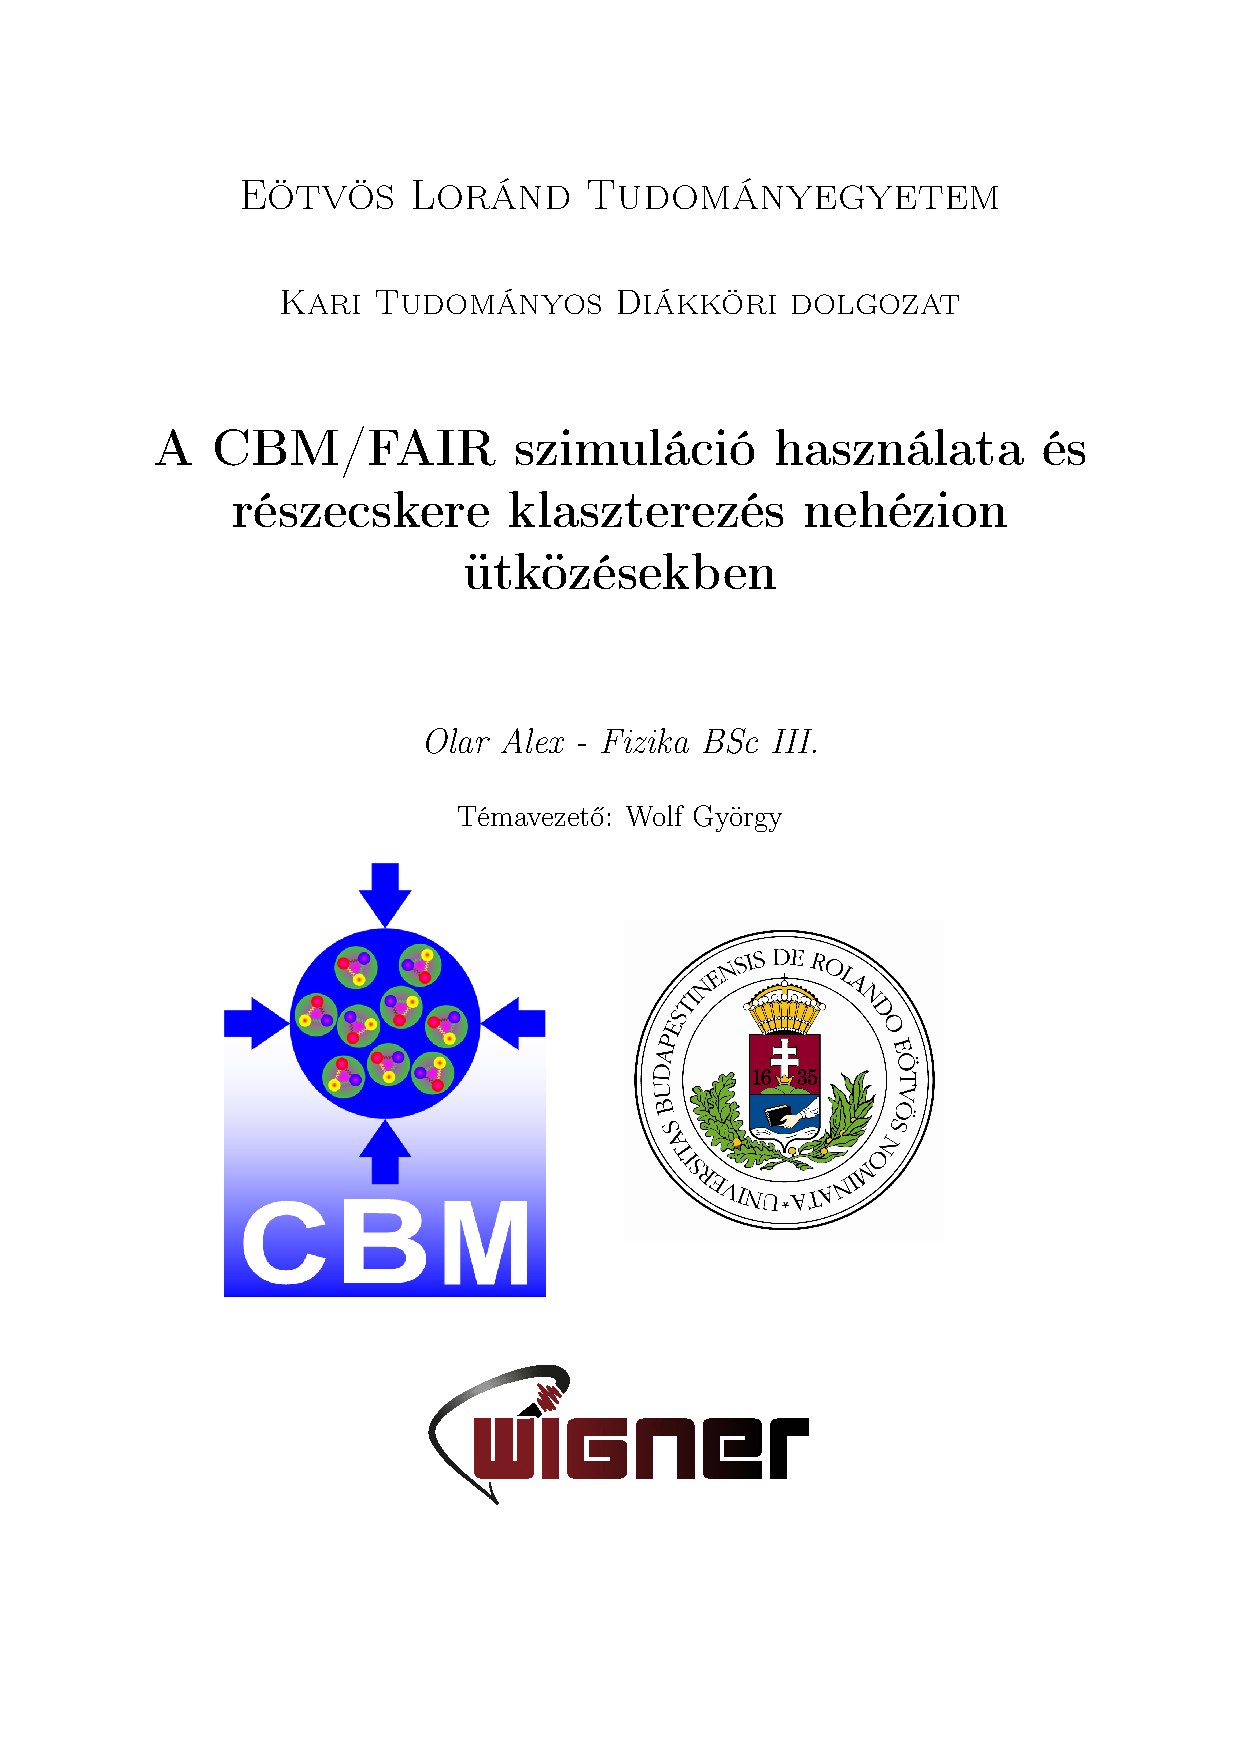
\includepdf{gsiTitlePage.pdf}
\begin{abstract}
	\par Egy hónapot töltöttem a nyár folyamán, július hónapba, Darmstadtban a GSI nevű kutatóközpontban. Kint tartózkodásom célja az volt, hogy többet megtudjak a  CBM saját szimulációjáról, amely kutató csoport már az
	 épülő FAIR\footnote{ Facility for Antiproton and Ion Research } része. Ezalatt a hónap alatt megismerkedtem mélyebben a ROOT \footnote{ CERN szoftver részecske analízishez} nevű szoftverrel, a
	  helyi cbmROOT-tal \footnote{ CBM ( Compressed Barionic Matter  ) szoftver a CBM/FAIR által fejlesztve}, valamint a C és C++ programozási nyelvekkel.
	\vspace{5mm}
	\par A kint létem alatt sokat tanultam a detektor technológiákról, valamint az azokban lejátszódó eseményekről.
	\vspace{5mm}
	\par Itthoni munkám során a nehézion ütközések szimulációjához kapcsolódva egy klaszterező program fejlesztésével foglalkoztam, 
	ami a kinyert adatokat csoportosítja térbeli és impulzustérbeli távolságuk alapján, előre definiált klaszterezési mérettel, az MST algoritmus felhasználása segítségével.
\end{abstract}
\tableofcontents
\section{ Alapok}
\subsection{ QCD - BSc-s szemmel}
\vspace{5mm}
\par A 20. század folyamán fizikusok szembesültek azzal, hogy milyen abszolút fontos szerepet töltenek be a szimmetriák az univerzum és a körülöttünk lévő világ
 megismerésében, miután a megmaradási tételekből következtettek rájuk.
\vspace{5mm}
\par A kvarkok felfedezése végre rendet teremtett a részecske állatkertben (particle ZOO), ahogy az elemi részecskék folyamatosan növő számára Niels Bohr szellemesen referált.
 A mennyiséget ami a különböző kvarkokat bizonyos szempontból jellemzi $\textsl{íz}$nek hívjuk, kezdetben
csak három kvarkíz volt ismert, úgy mint: $\textsl{u}$ (up), $\textsl{d}$ (down), $\textsl{s}$ (strange).
 A hadronok két csoportba oszthatók szét: $\textsl{mezonok}$ és $\textsl{barionok}$, amelyek rendre 
 egy kvark-antikvark párt vagy három kvarkot tartalmaznak.
\vspace{5mm}
\par Az erős kölcsönhatás, ami a kvarkok között ható elemi kölcsönhatás, egyedi tulajdonsága a bezárás, ami megakadályozza a kvarkokat abban, hogy elszeparálva,
 izoláltan megtalálhatóak legyenek. Az erős kölcsönhatás töltését színnek hívjuk. A bezárás miatt, az elemi részecskék csak úgynevezett semleges színben létezhet, amit gyakran `fehérnek' nevezünk. 
Az erős kölcsönhatást leíró alapvető elmélet a Kvantumszíndinamika (Quantum Chromo Dynamics) - QCD.
\vspace{5mm}
\par A QCD elemi részecskéi a kvarkok és antikvarkok, amelyek a gluonok által hatnak kölcsön, melyek szintén
 színtöltést hordoznak. A gluonoknak 8 fajtájuk van, hogy minden színtranszformáció leírható legyen segítségükkel. A gluonok önmagukkal is kölcsön tudnak hatni.
\subsection{ CBM fizika }
\vspace{5mm}
\par A barionanyaggal foglalkozva az elsődleges cél, hogy megértsük és jobban megismerjük a fázisdiagramot és magukat az átmeneti folyamatokat.
Először is rövid bevezetőként egy kis termodinamikai áttekintéssel kezdek a fázisokról és a fázisátalakulásokról, alapul véve a The CBM Book-ot:
\vspace{5mm}
\par A víz fázisdiagramja megmutatja annak különböző fázisait egy nyomás-hőmérséklet diagramon. Ismeretes, hogy adott körülmények között van egy
hármaspont, amelyben a víz mindhárom halmazállapotában előfordul. A fázisok közötti vonalak mentén a víz szintén több (itt kettő) halmazállapotban
előfordulhat és ezek mindketten megtalálhatóak a megfelelő körülmények között. Elsőrendű fázisátmenetnek hívjuk, amikor ezen vonalakon `áthaladva' halmazállapot-változás
történik. Továbbá megkülönböztetünk egy kritikus pontot is, amely után a fázisok nem különülnek el jelentős mértékben, ezután
csak egy úgynevezett sima $\textsl{crossover}$ figyelhető meg, nem elsőrendű fázisátmenet.
\begin{figure}[H]
	\centering
	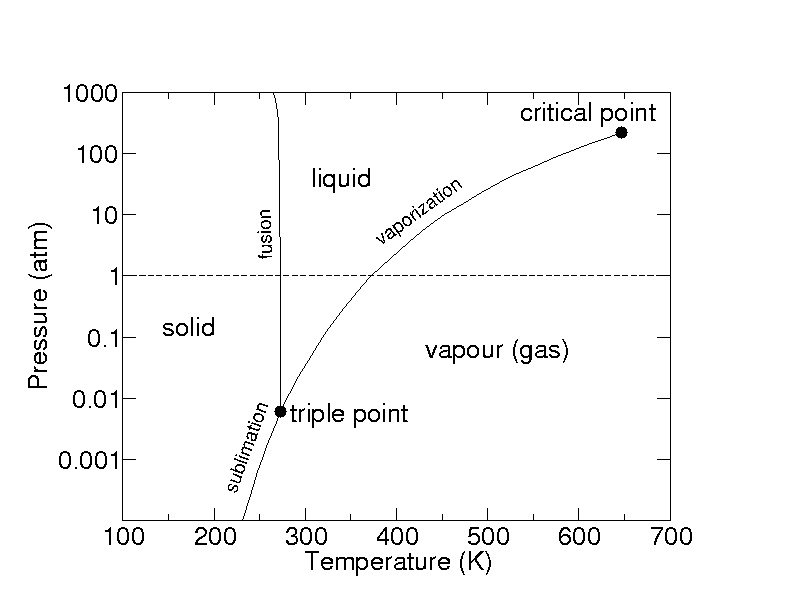
\includegraphics[width=0.76\textwidth]{water_phase.jpg}
	\caption{ A víz fázisdiagramja. }
\end{figure}
\par Most, hogy gyorsan áttekintettem a víz fázisdiagramját, vagy legalábbis egy részét, ideje továbblépni és feltenni a kérdést, hogy mi 
a helyzet az erősen kölcsönható anyaggal. Az erősen kölcsönható anyag fázisdiagramja ugyanis elméleti stádiumban van, még nincs teljesen feltárva.
Az ábrákon olyan különböző és elengedhetetlenül fontos fázisok vannak, amelyek a korai univerzumot jellemezték vagy éppen
a neutron csillagok anyagát alkothatják. Itt mindkét ábrán egy hőmérséklet-sűrűség diagramot láthatunk.
\begin{figure}[H]
	\centering
	\begin{subfigure}{.49\textwidth}
		\centering
		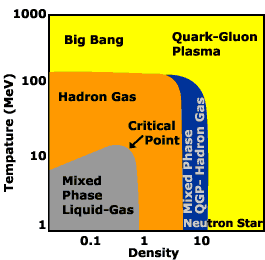
\includegraphics[width=0.92\textwidth]{cbm_phase1.png}
		\caption{ Hőmérséklet MeV-ban kifejezve, míg a sűrűség magsűrűségben van megadva, mindkét skála logaritmikus }
	\end{subfigure}
	\begin{subfigure}{.49\textwidth}
		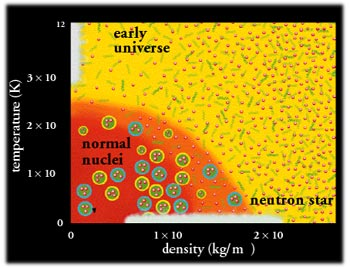
\includegraphics[width=.92\textwidth]{cbm_phase2.jpg}
		\caption{ Ezen a diagramon a fázisok természetbeli előfordulását láthatjuk. }
	\end{subfigure}
\end{figure}
\par A fentebbi ábrákon is látható egy fázis, amit kvark-gluon plazmának nevezünk. Ez az állapot jelen volt a Nagy Bummnál, de később
nem maradt fenn, a hőmérséklet hirtelen csökkenése miatt. Látható az is, hogy a neutron csillagok belseje is kvark-gluon plazmát tartalmazhat,
de azokban nem a hőmérséklet kell igen magas legyen, hanem a csillag sűrűsége. 
\vspace{5mm}
\par Nyilvánvalóan, a kvark-gluon plazma földi megfigyelésének egyetlen lehetőségét a nagy energiás részecskegyorsítók és azok
ütköztetése biztosítja. A QCD jellemző tulajdonsága, hogy a kvarkok közti összetartás csökken, ahogy az ütközési energiát
növeljük, ez az aszimptotikus szabadság jelensége. A részecskefizika egy másik fontos
szimmetriája a kiralitással kapcsolatos. Ez lényegében azt jelenti, hogy egy tömegtelen részecske spinje és sebességének iránya egymáshoz 
képest milyen irányba mutat. Hogyha azok egyirányúak, akkor a részecske jobb kezes, ha ellentétes irányúak akkor pedig bal kezes. Mivel
az up és down kvarkok tömege közel azonos és igen kicsi (nagy energiákon jó közelítéssel 0)
ezért azt szokták mondani, hogy a QCD-nek körülbelüli királis szimmetriája van. Ellenben, ez spontán
sérülhet alacsony hőmérsékleteken és sűrűségeken a párkölcsönhatások miatt. Emiatt az egyik királis irány ekkor 
gyakoribb lesz, mint a másik, ezt nevezzük lényegében királis szimmetriasértésnek. 
\section{ A CBM detektor}
\subsection{ Elmélet}
\vspace{5mm}
\par A nehézionok ütközésének vizsgálata és az adatok feldolgozása egy borzasztóan komplex feladat a reakció tranziens természete miatt. 
Lényegében az a cél, hogy az ütközés során, $10^{-22}~s$-ig fennálló állapot segítségével következtessünk az erősen kölcsönható anyag 
fázisdiagramjára, a jelenség természetére. Az idő természetesen nagyon rövid, és az egész jelenség csak a melléktermékek révén vizsgálható. 
\par  Az elmúlt évtizedben a fő tudományos tevékenység a témában a brookheaven-i RHIC  \footnote{ Relativistic Heavy Ion Collider - Brookhaven } központban 
és a CERN-ben található LHC \footnote{ CERN - Large Hadron Collider } gyorsítónál zajlott. Ezek a központok nagyon fontos, és érdemleges 
adatot biztosítanak a fázisdiagram vizsgálatához. Ellenben ezek mind az alacsony sűrűségű régiót vizsgálják és csak az aszimptotikus szabadságot tudják
feltérképezni a hadron gáz és a kvark-gluon plazma között. A FAIR projekt ezekkel szemben sokkal magasabb barion sűrűséget tervez elérni, hogy 
lehetőséget biztosítson az első rendű fázisátmenet vizsgálatára, valamint a kritikus pont környékének feltérképezésére. 
\begin{figure}[H]
	\centering
	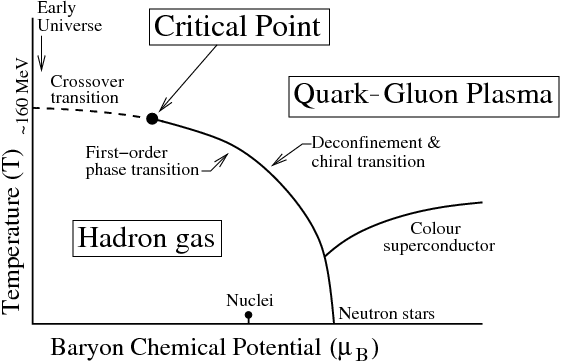
\includegraphics[width=0.96\textwidth]{CBM_phase_trans.png}
	\caption{ A fentebb említett elméleti fázisdiagram  }
\end{figure}
\subsection{ Detektor elrendezés és a szimuláció}
\par A detektor elrendezése balról jobbra haladva a következő (ábra):
\begin{itemize}
	\item CBM szupravezető mágnes szilícium spektrométerrel
	\item a micro vertex detektor ( MVD ) az előbbi belsejében
	\item a szilícium követő rendszer ( STS ) is
	\item Cserenkov-detektor ( RICH - ring imaging Cherenkov detector - világos kék )
	\item müon sprektrométer ( fekete )
	\item ezt követi 4 réteg átmeneti sugárzás ( TRD - transition radiation detector ) detektor
	\item és egy time-of-flight ( TOF ) fal
	\item a fő detektorok után található még  egy célfigyelő detektor (PSD)  
\end{itemize}
\begin{figure}[H]
	\centering
	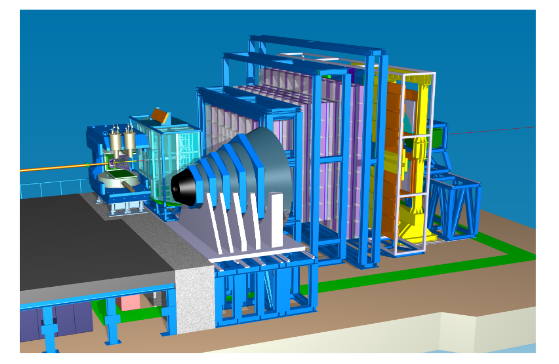
\includegraphics[width=0.66\textwidth]{cbm_detector.png}
	\caption{ A detektor elrendezés }
\end{figure}
\par A szilícium követő rendszer feladata az, hogy rekonstruálja majd a részecskék trajektóriáit. Csak töltött részecskék észlelésére képes, 
de képes mérni a töltés nagyságát és az impulzust is tud mérni. A TOF fal igen nagy felbontást tud elérni, nagyjából 60 ps-os felbontásra is
lehetőség van.
\vspace{5mm}
\par A CBM projekt még egyenlőre csak terv szintjén létezik, a szimulációt folyamatosan fejlesztik. Jövőre, vagy legkésőbb 2019-re már tervben 
van egy miniCBM detektor építése az esetleg később felmerülő tervezési, kivitelezési problémák elkerülésére. A FAIR létesítmény építése idén 
nyáron kezdődött és az első részecskenyaláb 2022-ben várható. A miniCBM projekt a meglévő GSI gyorsítónál fog tevékenykedni az addig fennmaradó
időben, ahol megpróbálják a számítógépfarmot tökéletesíteni, hogy az adatokat minél gyorsabban feldolgozhassák.
\vspace{5mm}
\par A FAIR tudósai kifejlesztettek egy több tízezer soros szimulációt, ami a ROOT-on alapszik. Ezt ők cbmROOT-nak hívják, mivel teljes
egészében a CBM-hez igazodik és ingyenesen elérhető bárki számára. Sok jól ismert nehézion szimulációs eljárást használnak, amik a CBM
környezetre vannak szabva, úgy mint: UrQMD \footnote{ Ultra Relativistic Quantum Molecular Dynamics }, valamint  PHSD \footnote{ Parton Hadron String Dynamics }.
 Ezek a szimulációs kódok széles körben használtak nem csak itt, hanem az egész nehézion fizika területén. 
\section{ A $\Phi$-mezonról röviden}
\subsection{ $\Phi$-mezon rekonstrukció}
\vspace{5mm}
\par A CBM detektor egy általános célú nehézion mérési eszköz lesz, hogy az erősen kölcsönható anyag fázisdiagramját vizsgálni lehessen. A
rezonanciák nagyon fontosak, hogy a sűrű anyagot vizsgálni tudjuk az ütközés során. Az ilyen rezonanciák egyike ami fontos a CBM és a 
fázisdiagram vizsgálatának szempontjából pedig a $\Phi$-mezon, aminek nagyon kicsi a hadronokra vett hatáskeresztmetszete így eléggé 
valószínűtlen, hogy kölcsönhat a nagy mennyiségű hadronnal, ami a reakció során keletkezik, vagyis jó indikátora a sűrű, kezdeti eseménynek.
A $\Phi$-mezon egy strange és egy anti-strange kvarkot tartalmaz és a kulcsa lehet az s kvark partonikus anyagban lévő keletkezésére. A
$\Phi$-mezon $K^{+}, K^{-}$ párokra bomlik nagyjából 50$\%$-os eséllyel és egyebekre (pl. dileptonokra is). A közepes élettartama egészen
kicsi a az ütközés idejéhez képest, nagyjából $1.55\cdot10^{-22}$ s tehát még a TOF falat sem éri el, csak a bomlástermékei lesznek detektálva már korábban is. 
A tömege $1.019$ MeV ami a kaonok invariáns tömegével kifejezve egy rezonancia csúcsként látható az ütközés/szimuláció után kinyert 
adatok között. Ahol a kaonok invariáns tömege:
\begin{equation*}
M_{KK} = \sqrt{(E_{1}+E_{2})^{2} - (\underline{p}_{1} + \underline{p}_{2})^{2}}
\end{equation*}
\vspace{5mm}
\par Én a PHSD adatait vizsgáltam, amin lefuttattam a CBM szimulációt. Egy Au+Au centrális ütközést vizsgáltam $10$ GeV-es bombázó energián. 
A CBM szimuláció kimenetét a cbmROOT-tal rekonstruáltam. Több mint 5 millió esemény szerepelt a kezdeti $.root$ fájlban amit a szimulációhoz 
használtam.
\vspace{5mm}
\par A hisztogramokon az x-tengelyen a kaon párok invariáns tömege szerepel, az y-tengelyen pedig az adott energián a `beütések' száma. Egy 
apró kiugrás látható a nagy kombinatorikus háttéren nagyjából $1.02$ GeV környékén ami pontosan a $\Phi$-mezonok bomlásából adódik.
\begin{figure}[H]
	\centering
	\begin{subfigure}{0.49\textwidth}
		\centering
		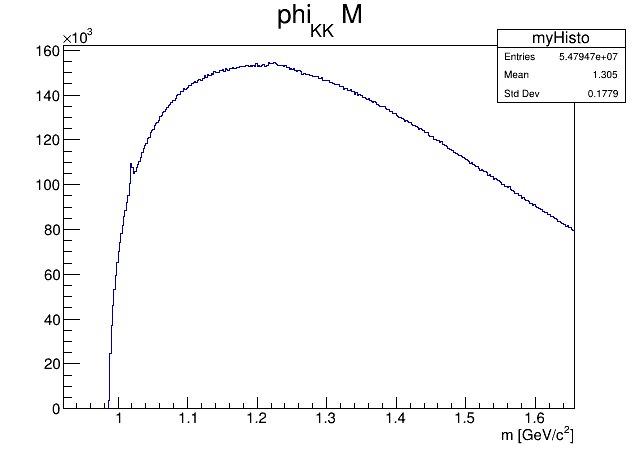
\includegraphics[width=0.95\textwidth]{phi_KK_M.png}
		\caption{ A kombinatorikus háttér és egy apró, de jól látható csúcs. }
	\end{subfigure}
	\begin{subfigure}{0.49\textwidth}
		\centering
		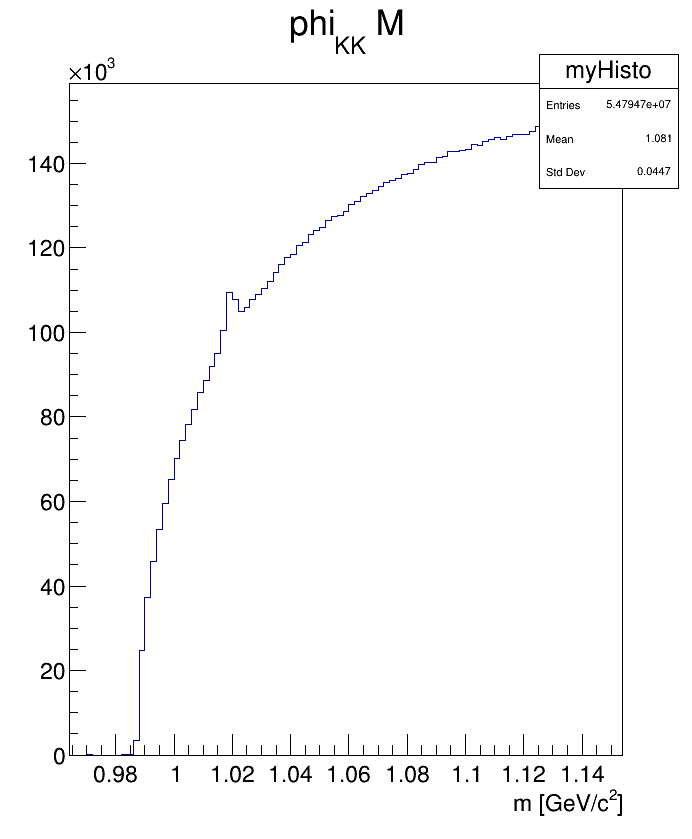
\includegraphics[width=0.95\textwidth]{phi_KK_Mzoom.png}
		\caption{ A csúcs. }
	\end{subfigure}
\end{figure}
\par Egy másodfokú polinommal próbáltam becsülni a hátteret. Az illesztés paraméterei ($ax^{2} + bx +c$) :
\begin{center}
	\begin{tabular}{|c|c|c|}
		\hline
		Parameter name & Value []     & Error   \\
		\hline
		a              & -7.70559e+06 & 78750.5 \\
		\hline
		b              & 1.42738e+07  & 150055  \\
		\hline
		c              & -6.49147e+06 & 71438.9 \\
		\hline
	\end{tabular}
\end{center}
\par A háttér illesztése: 
\begin{figure}[H]
	\centering
	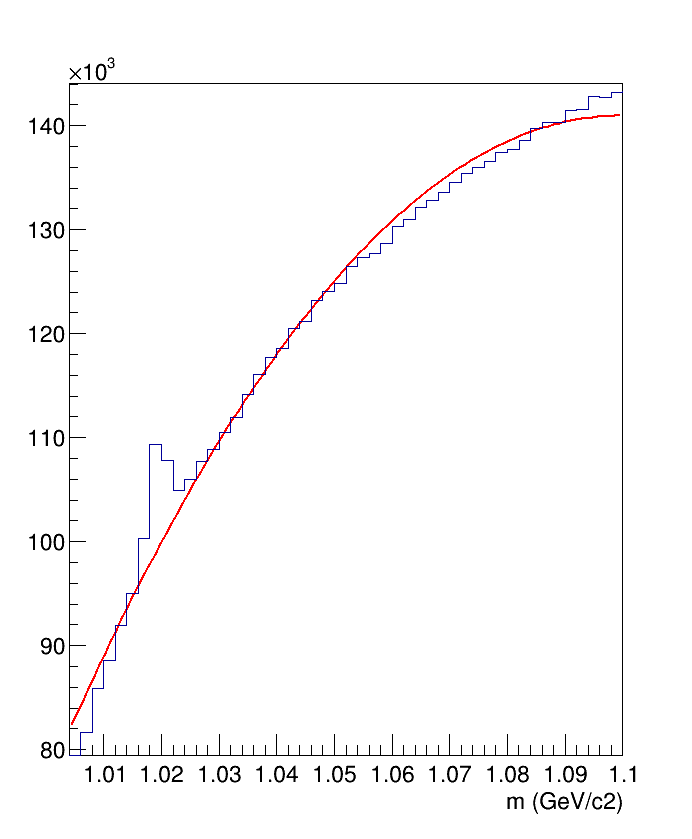
\includegraphics[width=0.35\textwidth]{combiback_fit.png}
	\caption{ A háttérre vett illesztés a másodfokú polinommal. }
\end{figure}
\par A csúcs közelítéséhez más módszert alkalmaztam. Egy alacsony multiplicitású jelet használtam a csúcs alakjának becsléséhez, amit egy
Gauss-függvénnyel illesztettem, majd ezt skáláztam fel a csúcshoz, az állandó nagyságú háttér mellett, az eredmények a következők:
\begin{figure}[H]
	\centering
	\begin{subfigure}{0.49\textwidth}
		\centering
		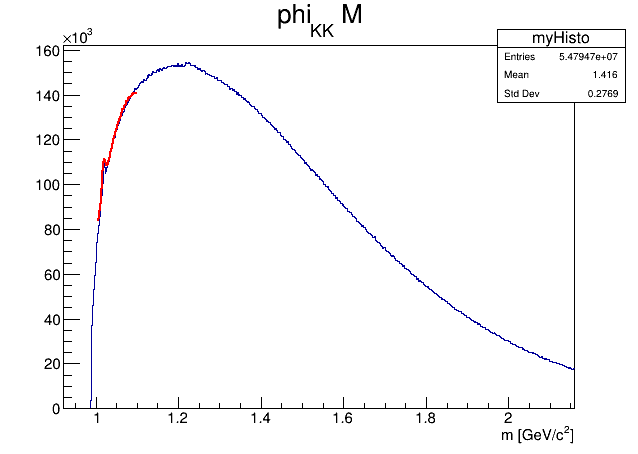
\includegraphics[width=0.95\textwidth]{phi_KK_Mfit.png}
		\caption{ A háttér és a csúcs illesztése. }
	\end{subfigure}
	\begin{subfigure}{0.49\textwidth}
		\centering
		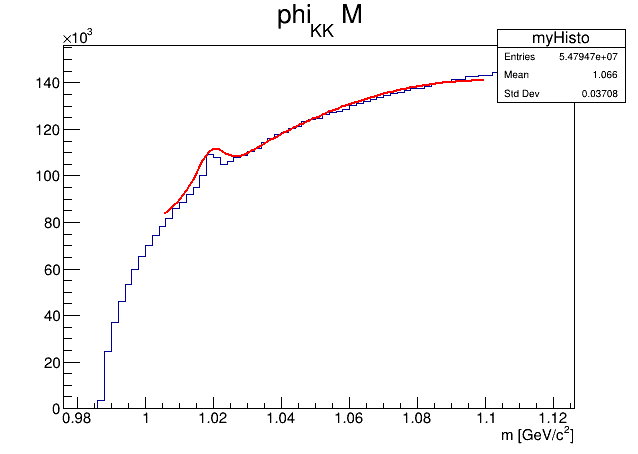
\includegraphics[width=0.95\textwidth]{phi_KK_Mfitzoom.png}
		\caption{ Ráközelítve. }
	\end{subfigure}
\end{figure}
\par Itt a ROOT makróm, amit az `illesztéshez' használtam:
\lstinputlisting[language=C++]{fit.C}
\par Ez nem igazán pontos közelítés, de jól szemlélteti, hogy a háttér jól közelíthető ellenben ekkora számú eltérés már megmutatkozik benne.
\subsection{$\Phi$-mezon a CBM-ben}
\vspace{5mm}
\par Igen nehéz feladat lesz hatékonyan detektálni a $\Phi$-mezonokat a CBM detektorrendszerrel. A részecskék nem csak rövid 
életűek, de egy hatalmas háttér is nehezíti az apró csúcs megtalálását. Ezért is kell hatalmas számú eseményt vizsgálni, hogy a csúcs
a statisztikában már látható legyen. Ennek ellenére határozottan mondhatjuk, hogy a CBM detektor képes lesz a $\Phi$-mezonok detektálására
és ezáltal a strange kvark termelődésének megértésére az erősen kölcsönható anyagban.
\vspace{5mm}
\par A szimuláció hatékonysági mutatókat is biztosít. Mindezeket különböző részecske impulzusok esetén. A jelzett detektálás 
hatékonysági értékek nem túl magasak, de eléggé stabilak adott tartományokban az észleléshez:
\begin{figure}[H]
	\centering
	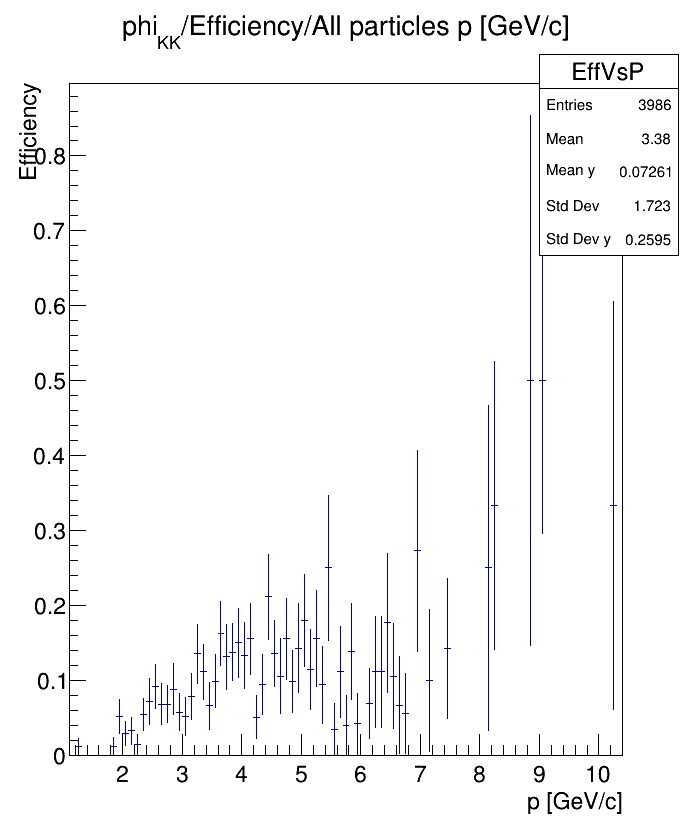
\includegraphics[width=0.65\textwidth]{efficieny.png}
	\caption{ Hatékonyság az impulzus függvényében }
\end{figure}
\section{ A szimuláció}
\vspace{3mm}
\subsection{ Telepítés}
\vspace{5mm}
\par A CBM szimuláció telepítésének három fő komponense van, az egyik a FairROOT, majd a FairSoft és végül a cbmROOT. Bármilyen 
rendszerre telepíthetőek az alábbi linkről:
\url{https://redmine.cbm.gsi.de/projects/cbmroot/wiki/InstallCbmRootAuto} \newline
\par Erősen ajánlott a telepítést ezt követve megtenni, mivel rengeteg apró, de akadályozó probléma előjöhet a telepítés során. A teljes
csomag tartalmazza a ROOT-ot is, így az egész nagyjából 25 GB helyet foglal. 
\subsection{ Bevezetés}
\vspace{5mm}
\par Maga az ütközés a UrQMD és a PHSD programok segítségével játszódik le, a CBM szimuláció a detektor választ szimulálja, tehát az ezekből
származó adatokat kapja meg kezdeti paraméternek. Ezek a modellek az ALICE, RHIC és LHC detektornak, valamint nem utolsó sorban a
CBM detektornak lettek fejlesztve. Én főleg UrQMD adatokat használtam, de PHSD fájlokkal is találkoztam kint létem során. 
\vspace{5mm}
\par Az első lépés az, hogy le kell futtatni egy Monte Carlo szimulációt, hogy képeset legyünk a `valódi' adatokat összepárosítani a 
keltett eseményekkel. A program ezen része arra lett tervezve, hogy kiszűrje a találatokat a detektor anyagban és olyan pontokat találjon, 
amelyek később trajektóriákká összeállíthatók.
\vspace{5mm}
\par A program a Geant3 és Geant4 programokat használja, hogy a részecskék anyagon való áthaladását szimulálja. Ez is a Monte Carlo 
szimuláció része.
\vspace{5mm}
\par Az első makró kimenetén tehát egy szimulációs fájl van, ami az STS és az MVD detektorok által detektált találatokat tartalmazza 
valamint a TOF fal és egyéb detektorok adatait is. Ezeket felhasználva lép a program a második fázisba, a rekonstrukció részhez. A rekonstrukciós 
kód először is klasztereket próbál találni az MVD detektorban, hogy megtalálja, hogy hol volt az ütközés/ütközések kiinduló pontja. Ha ezt megtalálta
továbbhalad és megpróbálja lekövetni a részecske pályákat. A töltött részecskék körpályára állnak az erős mágneses tér hatására így a pontokra
köríveket próbálnak illeszteni és a legjobb illesztéssel bírókat fogadják csak el (van egy százalékos határ, ami alatt hibás detektálásnak ítélik). Én főleg
az MVD és STD detektorokra koncentráltam, tehát a többit most nem említem itt.
\vspace{5mm}
\par Nyilvánvalóan, a találatok és a pályákat többször próbálja meg a program helyesen megtalálni, azért, hogy elkerülje a hibákat. Kisebb
az esélye így a hibás találatnak, vagy a hibásan illesztett trajektóriának. Ennék része a digitalizáció, ami lényegében azt jelenti, hogy a 
szimulációs program megpróbálja a detektor választ is számításba venni. Vegyük például az STS detektort. Ennek egy szálas, hálós elrendezése 
van, amikor egy részecske áthalad, akkor több szálban is detektáljuk, ezek metszéspontjában van a tényleges helye. De ha egyszerre két
részecske ment át `ugyan azon a ponton', akkor ezt nem láthatjuk, később a pályák illesztésénél probléma lehet. Ezért is van az, hogy ha
az STS detektor több, mint 5$\%$-a detektál, akkor a rendszer lényegében nem mér, nem szerez kiértékelhető adatokat.
\vspace{5mm}
\par A sikeres rekonstrukció után, ami a nyers adatokból létrehozta végső soron a trajektóriákat az egyetlen visszamaradó feladat a 
részecske felismeres és ezek pályákhoz való párosítása. Erre egy robusztus és hatékony program áll rendelkezésre, aminek a neve KFParticleFinder.
\vspace{5mm}
\par Ennek a programnak a kimenete egy .root fájl, ami rengeteg részecskét és hozzájuk tartozó adatot tartalmaz, detektálási hatékonyságról,
háttérről, armenteros diagramokkal, bemenő és kimenő jelekkel, stb. . Az szerkezete nagyjából így néz ki:
\begin{figure}[H]
	\centering
	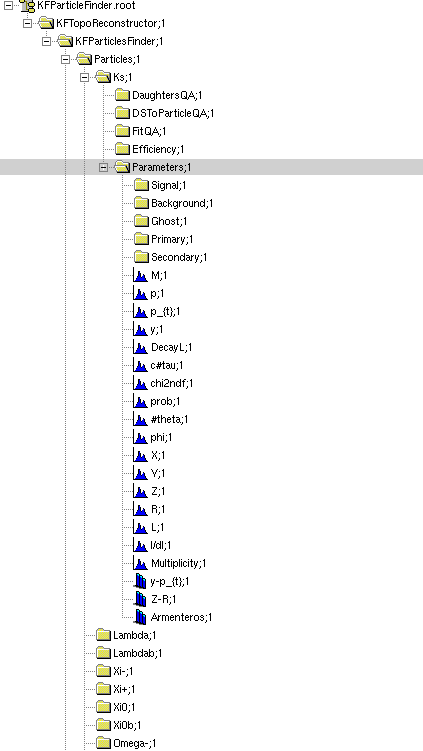
\includegraphics[width=0.42\textwidth]{particle_file.png}
	\caption{ A ROOT fájl struktúrájának egy része. }
\end{figure}
\vspace{5mm} 
\par 
\begin{figure}[H]
	\centering
	\begin{subfigure}{0.49\textwidth}
		\centering
		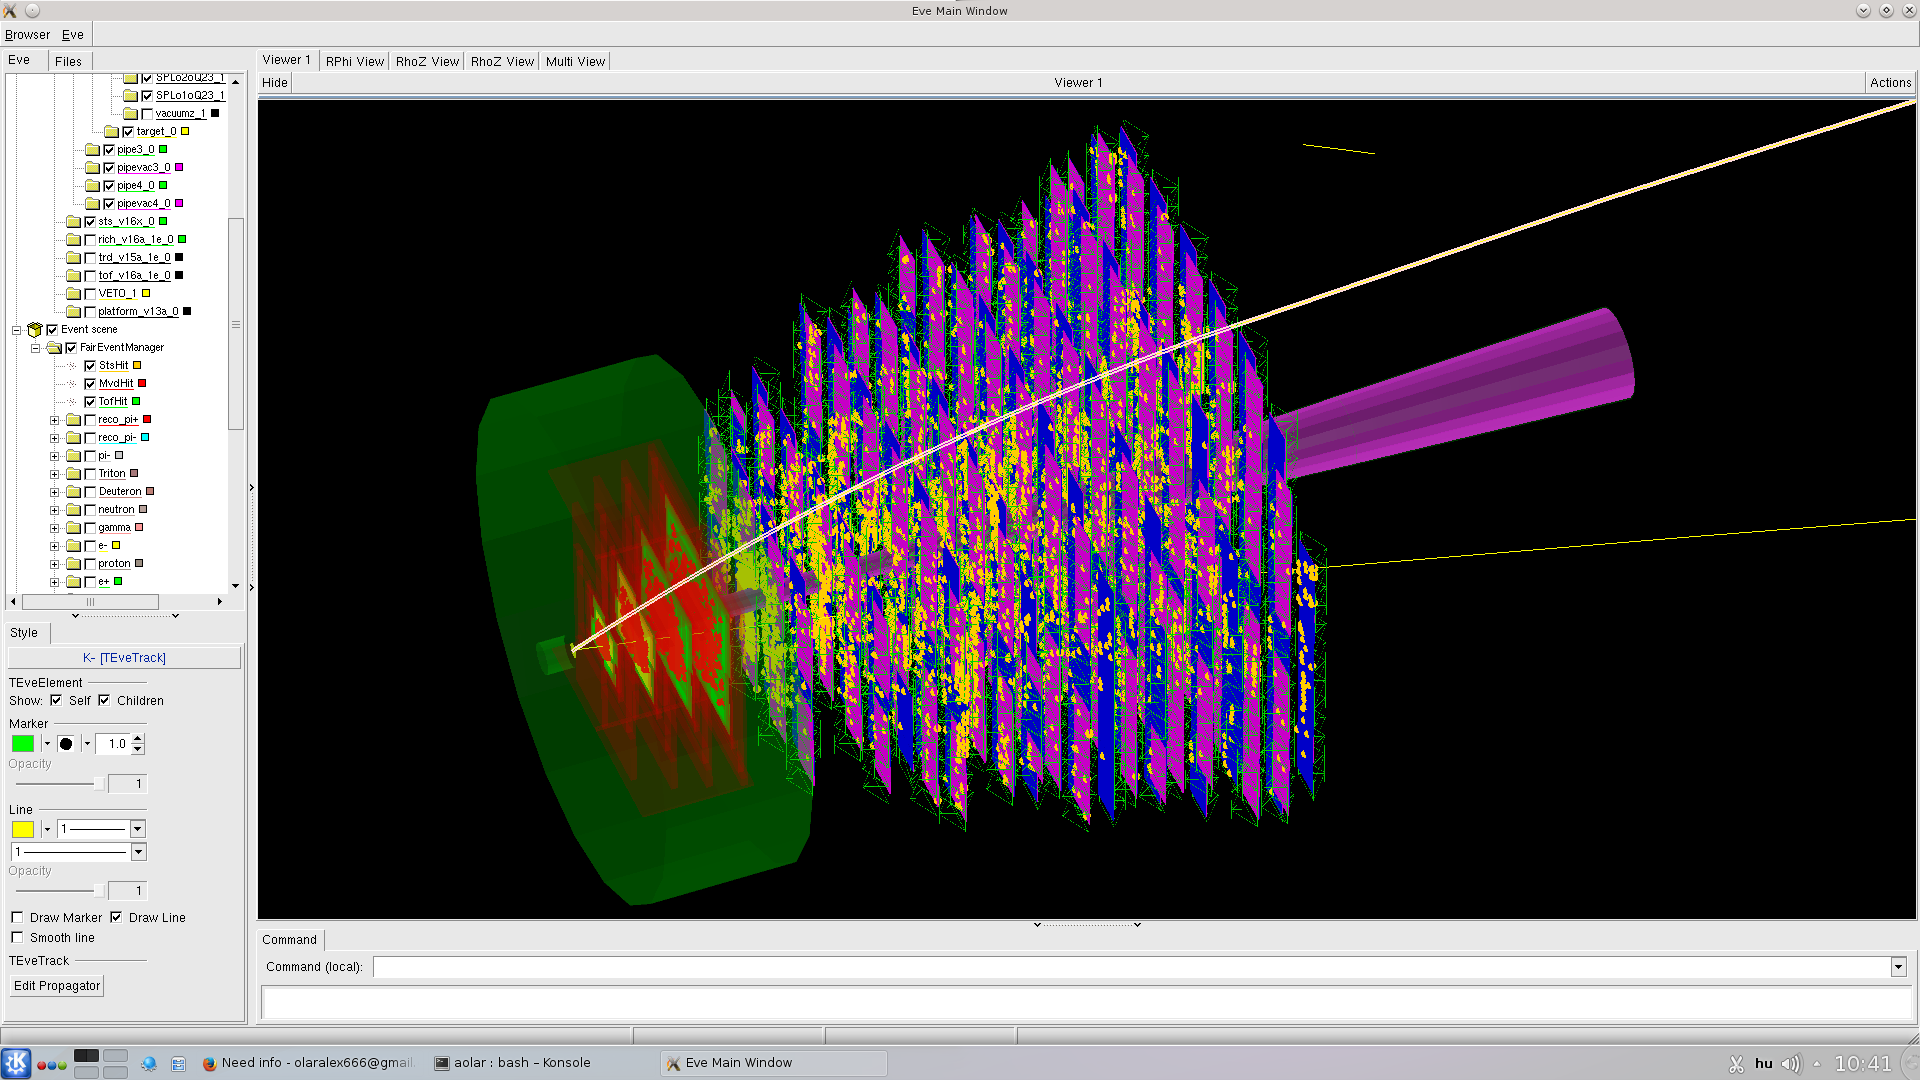
\includegraphics[width=0.95\textwidth]{reco2.png}
		\caption{ A rekonstruált pályák az MVD és STS detektorokban. }
	\end{subfigure}
	\begin{subfigure}{0.49\textwidth}
		\centering
		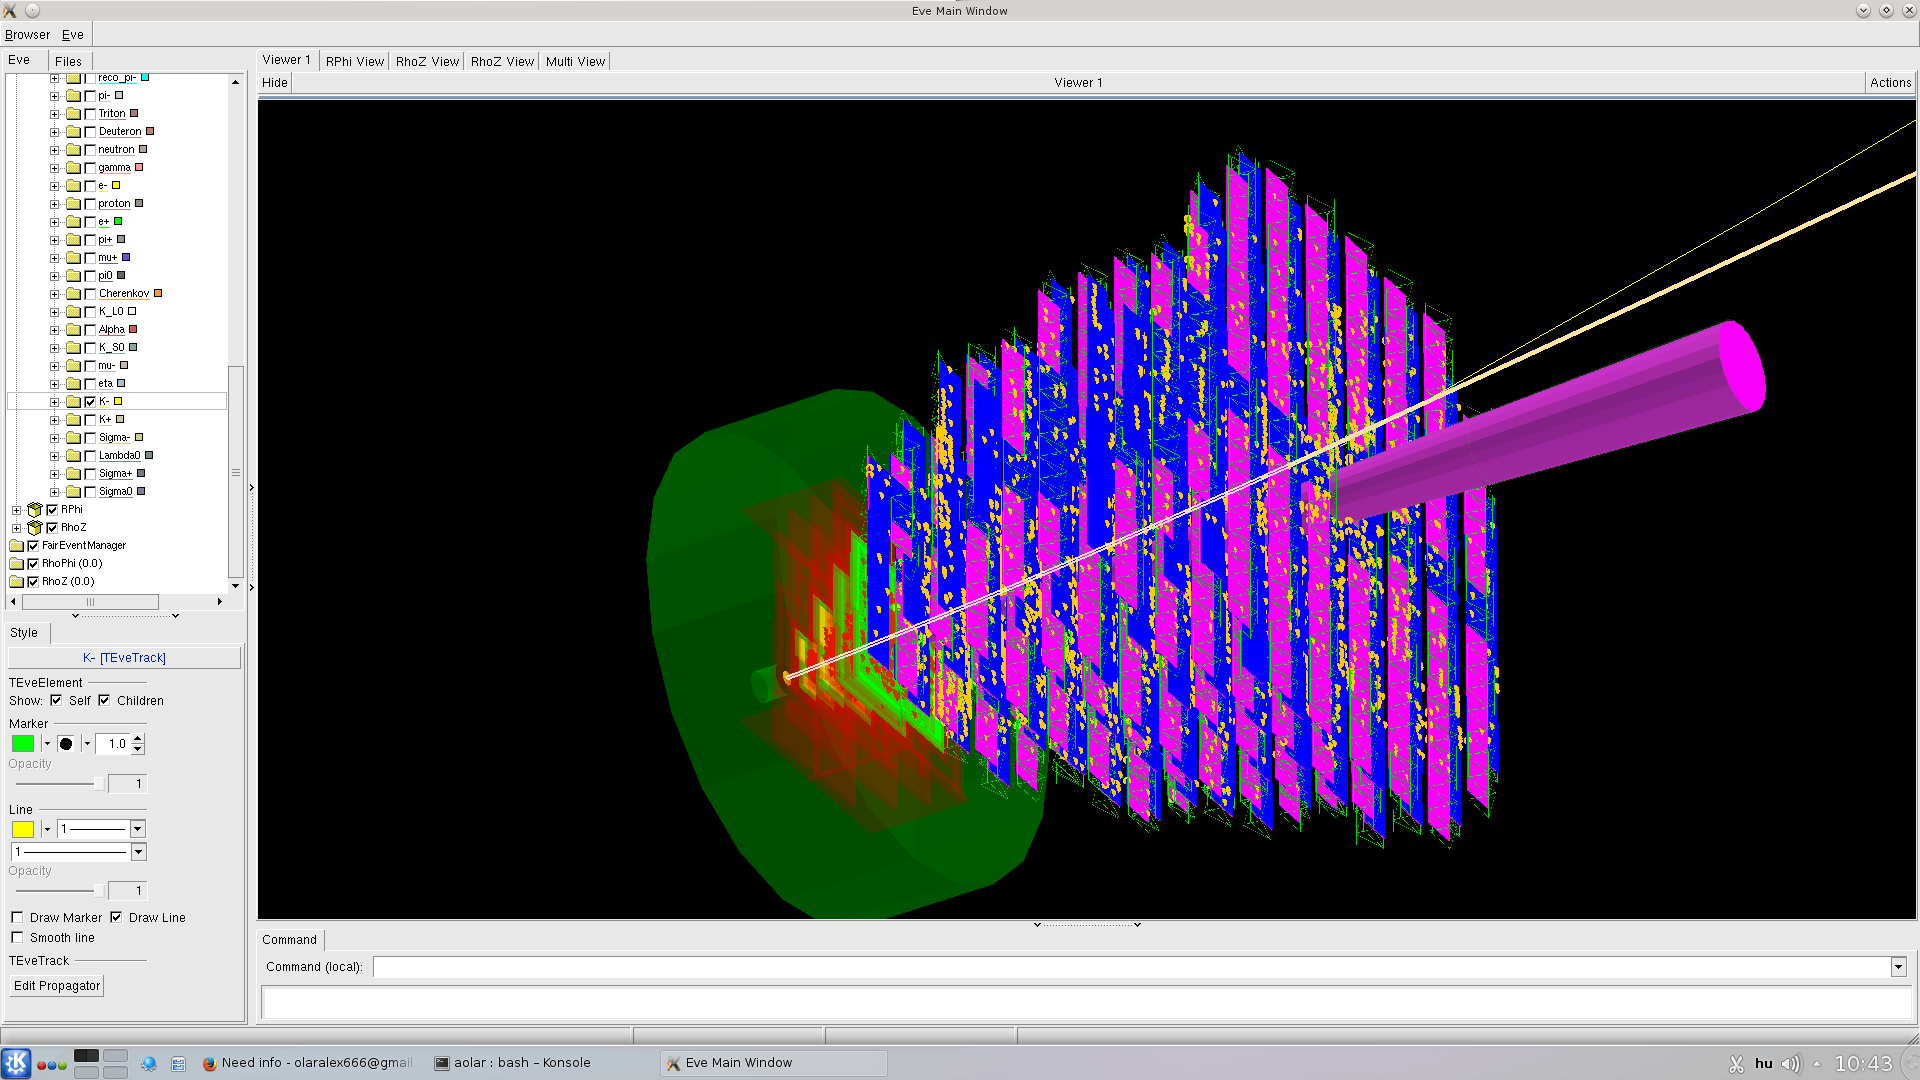
\includegraphics[width=0.95\textwidth]{reco1.png}
		\caption{ Másik szögből }
	\end{subfigure}
\end{figure}
\subsection{ How-tos}
\vspace{3mm}
\par Ahogy korábban említettem először a Monte Carlo szimulációt kell használni valamilyen bemeneti fájllal. Ez egy .root fájl vagy egy 
egyszerű ASCII fájl is lehet, a szimulációs kód képes mindkettő fogadására. Egy ilyen fájlban részecske ID-k és impulzusuk található. A kimenete 
a PHSD és a UrQMD szimulációknak általában egy .root fájl, de például a HIJING sima szöveges kimenetet produkál. A CBM szimulációnál különböző 
függvények teszik lehetővé mindkét adattípus feldolgozását.
\vspace{3mm}
\par Megtanultam használni a jelgenerátor programot, amivel bárki, bármit küldhet a detektor szimuláció bemenetére. Én főként arra használtam, hogy
kontrollált körülmények között, csak $\Phi$-mezonokat küldjek be, amivel vizsgálni lehet, hogy mi lesz a program kimenetén a KFParticleFinder
által kiadott .root fájlban. Ahhoz, hogy a generátor által biztosított ASCII fájlt olvasni tudja a szimuláció a következő módosítások szükségesek:
\begin{figure}[H]
	\centering
	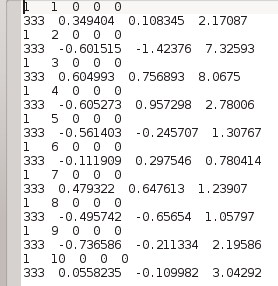
\includegraphics[width=0.5\textwidth]{input.png}
\end{figure}
\par 333 a részecske ID a $\Phi$-mezonnál. Ezután a szimuláció tudni fogja, hogy hogyan dolgozza azt fel, és képes lesz azt elbomlasztani
a megfelelő valószínűségekkel. 
\begin{lstlisting}[language=C++]
FairAsciiGenerator *SignalGen = new FairAsciiGenerator(inFile);
primGen->AddGenerator(SignalGen);
\end{lstlisting}
Fentebb a .root fájlokhoz használt $CbmUnigenGenerator$ helyett ASCII fájlok esetén ezt kell használni. Még egy fontos lépes van itt. Ha szeretnénk
vizualizálni a későbbiekben az eredményeinket, akkor engedélyeznünk kell a trajektóriák ilyen szintű mentését. Ez nyilvánvalóan nem 
hatékony hatalmas részecske számok esetén, de ha csak néhány részecskét küldünk be, akkor hasznos lehet látni, hogy hogyan is működik a 
program, esetleg hibákat is észrevehetünk.
\begin{lstlisting}[language=C++]
 // -Trajectories Visualization (TGeoManager Only )
 run->SetStoreTraj(kTRUE);  //->
 // -----------------------------------------------
\end{lstlisting}
\par Tehát a rekonstrukció után, valamint a részecske felismerés végeztével, ha bekapcsoltuk a vizualizációt képesek vagyunk vizualizálni az
eseményeket. Ehhez az $eventDisplay.C$ makrót kell futtatnunk. Ez a makró az egész CBM geometriát tartalmazza, tehát az egész 
detektort átláthatjuk vele. Megjeleníthető benne az összes trajektória és a részecskék. Néhány kép arról, ahogy egy $\Phi$-mezon két kaonra bomlott:
\begin{figure}[H]
	\centering
	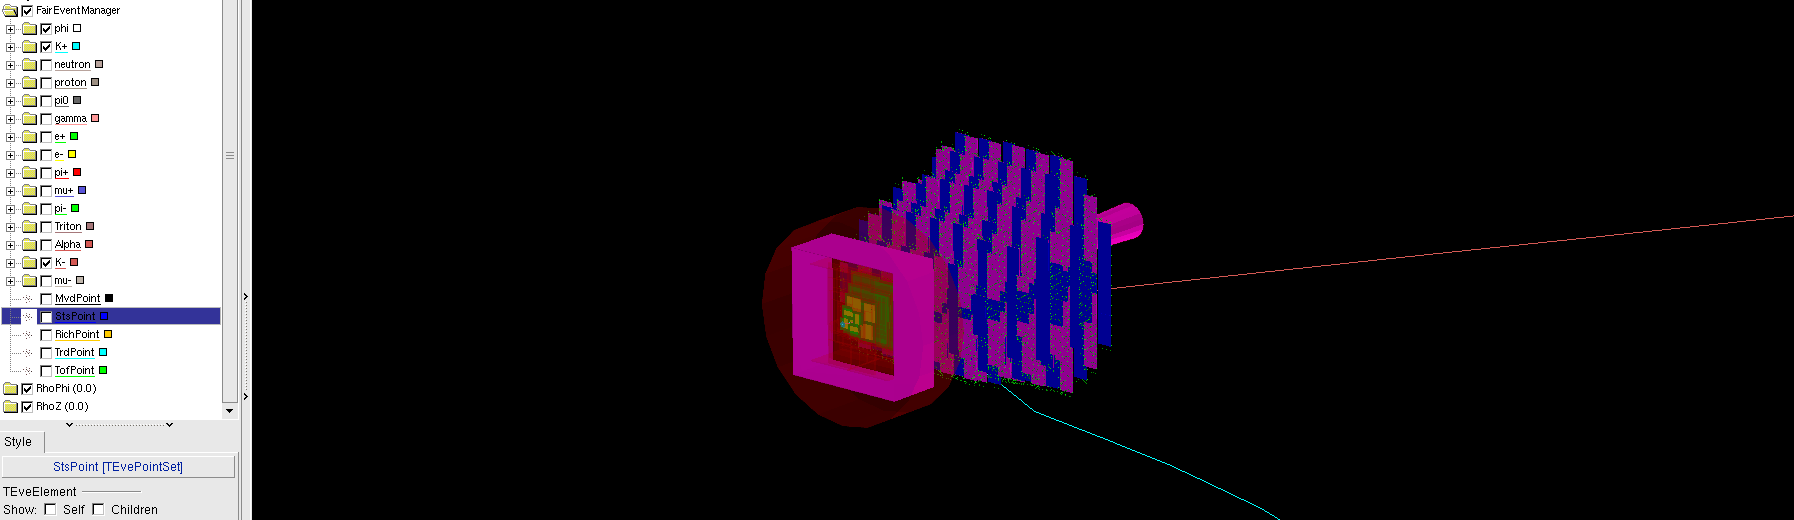
\includegraphics[width=0.85\textwidth]{k-k+decayofphi.png}
	\caption{ Vizualizáció az MVD és STS detektorokban }
\end{figure}
\subsection{ $\Phi$-mezonok generálása és a kimenő adatok elemzése}
\vspace{5mm}
\par A jelgenerátorral 2500 eseményt generáltam ahol a $\Phi$-mezonok pont a céltárgy közepében helyezkedtek el, tehát mintha éppen 
ott keletkeztek volna az ütközés során. Az ilyen adatok elemzése azért fontos, mert ekkor kontrollált körülmények között, adott részecske számmal
tudjuk vizsgálni a kimenő részeskék számát, eloszlását és ebből ismeretlen mennyiségű kezdeti részecskénél következtethetünk a $\Phi$-mezonok számára
így a strange keltés folyamatára. 
\par A generátor makróban a bemenő nyaláb energiáját is változtathatjuk, valamint a környezet hőmérsékletét is (mindkettő GeV-ben) és persze
azt is, hogy milyen részecskét akarunk generálni.
\begin{lstlisting}[language=C++]
double fSlope = .154; // temperature
...
double eBeam = 10.; // beam energy
double pBeam = TMath::Sqrt(eBeam*eBeam - kProtonMass*kProtonMass);
...
 const int NParticlesPerEvent = 1;
 const double kSignalMass[NParticlesPerEvent] = {1.019455};    //  mass in GeV
 const int    kSignalID[NParticlesPerEvent] =  {333};
 ...
   for (int i=0; i<NEvent; i++){
   // Generate rapidity, pt and azimuth
   outputfile<<NParticlesPerEvent<<"   "<<i + 1<<"  "<<0.<<"  "<<0.<<"  "<<0.<<endl;
   for(int j=0;j<NParticlesPerEvent;++j) {      
   double yD   = gRandom->Gaus(fYcm, fRapSigma);
   double ptD  = fThermal[j].GetRandom();
   double phiD = gRandom->Uniform(0., kTwoPi);
   
   // Calculate momentum, energy, beta and gamma
   double pxD    = ptD * TMath::Cos(phiD);
   double pyD    = ptD * TMath::Sin(phiD);
   double mtD    = TMath::Sqrt(kSignalMass[j]*kSignalMass[j] + ptD*ptD);
   double pzD    = mtD * TMath::SinH(yD);
   
   outputfile<<kSignalID[j]<<"  "<<pxD<<"  "<<pyD<<"  "<<pzD<<endl;
   
   }
   }
\end{lstlisting}
\par Jól látható, hogy ezt a makrót elég könnyű személyre szabni, tehát bárki könnyedén elkészítheti magának a számára megfelelő
bemeneti fájlt. A bemeneti fájlt az események számával és a fájl nevével át kell adni a szimulációs programnak.
\begin{lstlisting}[language=C++]
void run_mc_phi(TString inFile="Signal_phi_2500.txt", const char* setupName = "sis100_electron", Int_t nEvents = 2500)
{
  TString outFile = "sim_phi_2500.root";
  TString parFile = "param_phi_2500.root";
...
  // --- Define the target geometry -----------------------------------------
  //
  // The target is not part of the setup, since one and the same setup can
  // and will be used with different targets.
  // The target is constructed as a tube in z direction with the specified
  // diameter (in x and y) and thickness (in z). It will be placed at the
  // specified position as daughter volume of the volume present there. It is
  // in the responsibility of the user that no overlaps or extrusions are
  // created by the placement of the target.
  //
  TString  targetElement   = "Gold";
  Double_t targetThickness = 0.025;  // full thickness in cm
  Double_t targetDiameter  = 2.5;    // diameter in cm
  Double_t targetPosX      = 0.;     // target x position in global c.s. [cm]
  Double_t targetPosY      = 0.;     // target y position in global c.s. [cm]
  Double_t targetPosZ      = 0.;     // target z position in global c.s. [cm]
  Double_t targetRotY      = 0.;     // target rotation angle around the y axis [deg]
}
\end{lstlisting} 
\par A kimenet egy .root fájl, ami mint már korábban említettem adatokat tartalmaz a beütésekkel a detektor anyagban. Fontos megemlíteni, 
hogy a céltárgyat is bárminek definiálhatjuk, a helyzetét is változtathatjuk, de a mi feladatunk, hogy helyesen tegyük, mert a szimuláció lefut 
úgy is, hogy a nyaláb el sem találja a céltárgyat. 
\vspace{5mm}
\par Ezután a rekonstrukciós fájlt is kissé módosítani kell, majd ez a trajektóriákat találja meg. Majd a fizika makrót kell futtatni, hogy a 
KFParticleFinder megtalálja a pályákhoz tartozó részecskéket. A kimeneti .root fájlból néhány részlet:
\begin{figure}[H]
	\centering
	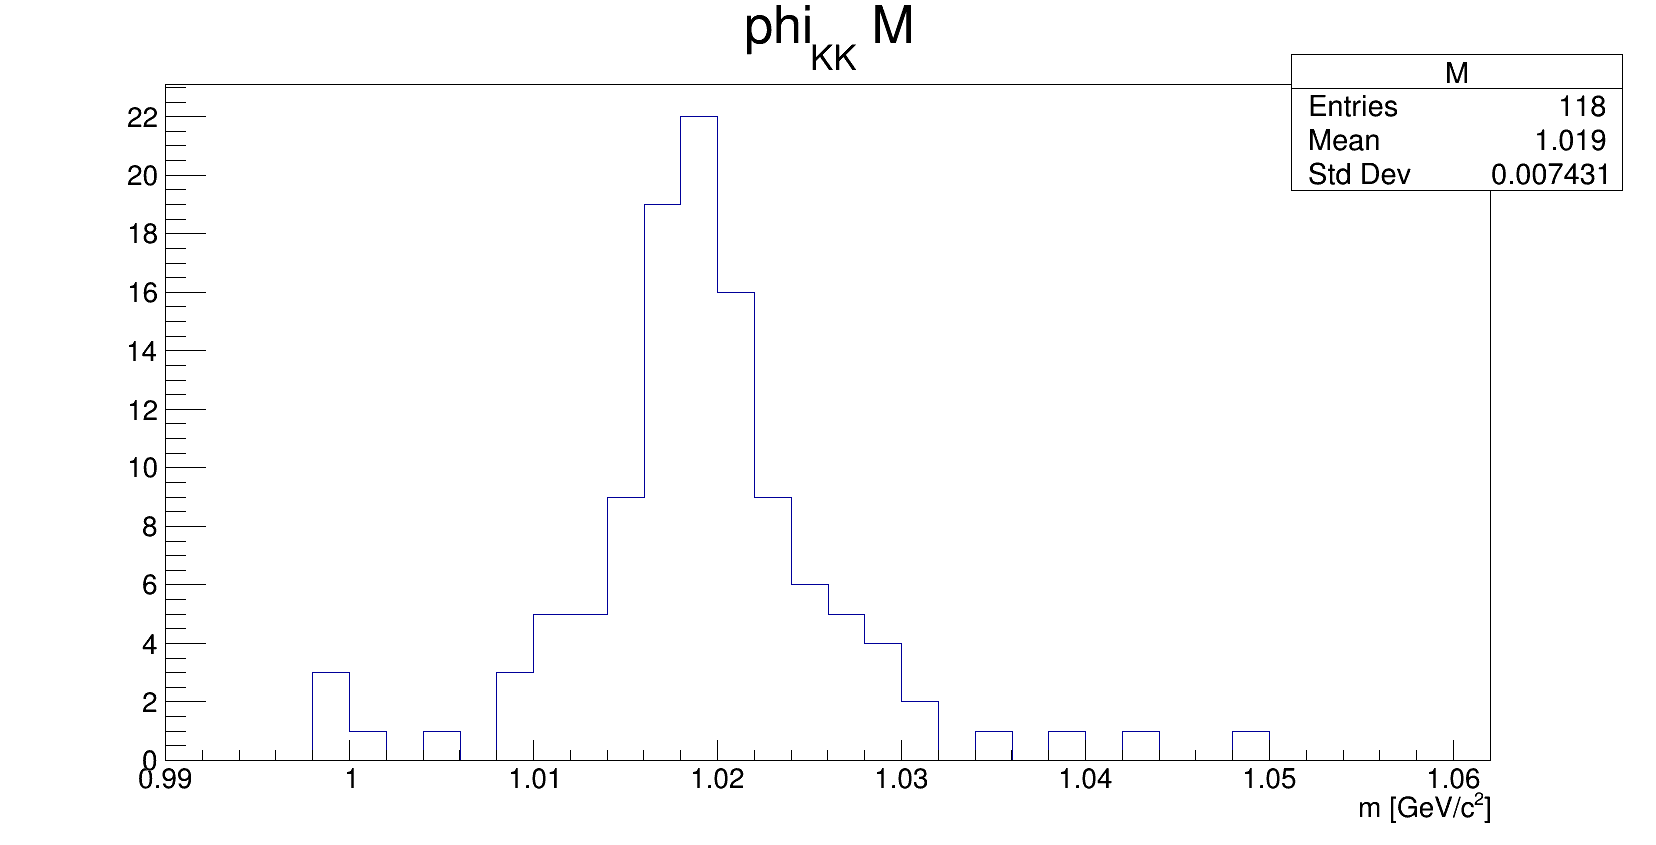
\includegraphics[width=0.5\textwidth]{phiKK_2500phi.png}
	\caption{ A kaonpárok invariáns tömegének diagramján 1.02 GeV-nél, a $\Phi$-mezon }
\end{figure}
\par A jelben 2500 esemény volt, azaz 2500 db mezont generáltam. Nagyjából 50$\%$-os eséllyel bomlottak el ezek kaon párokra, 
valamint a digitalizáció során, nagyjából 15$\%$-os hatékonysággal tudott a program rekonstruálni, azaz nagyjából 180 db rekonstruált
$\Phi$-mezonra lehet számítani a $KFParticleFinder.root$ fájlban. A fájlban ezzel ellentétben még csak 120 db-ot sikerült rekonstruálni, tehát
a szimuláció további tökéletesítésre szorul.
\begin{figure}[H]
	\centering
	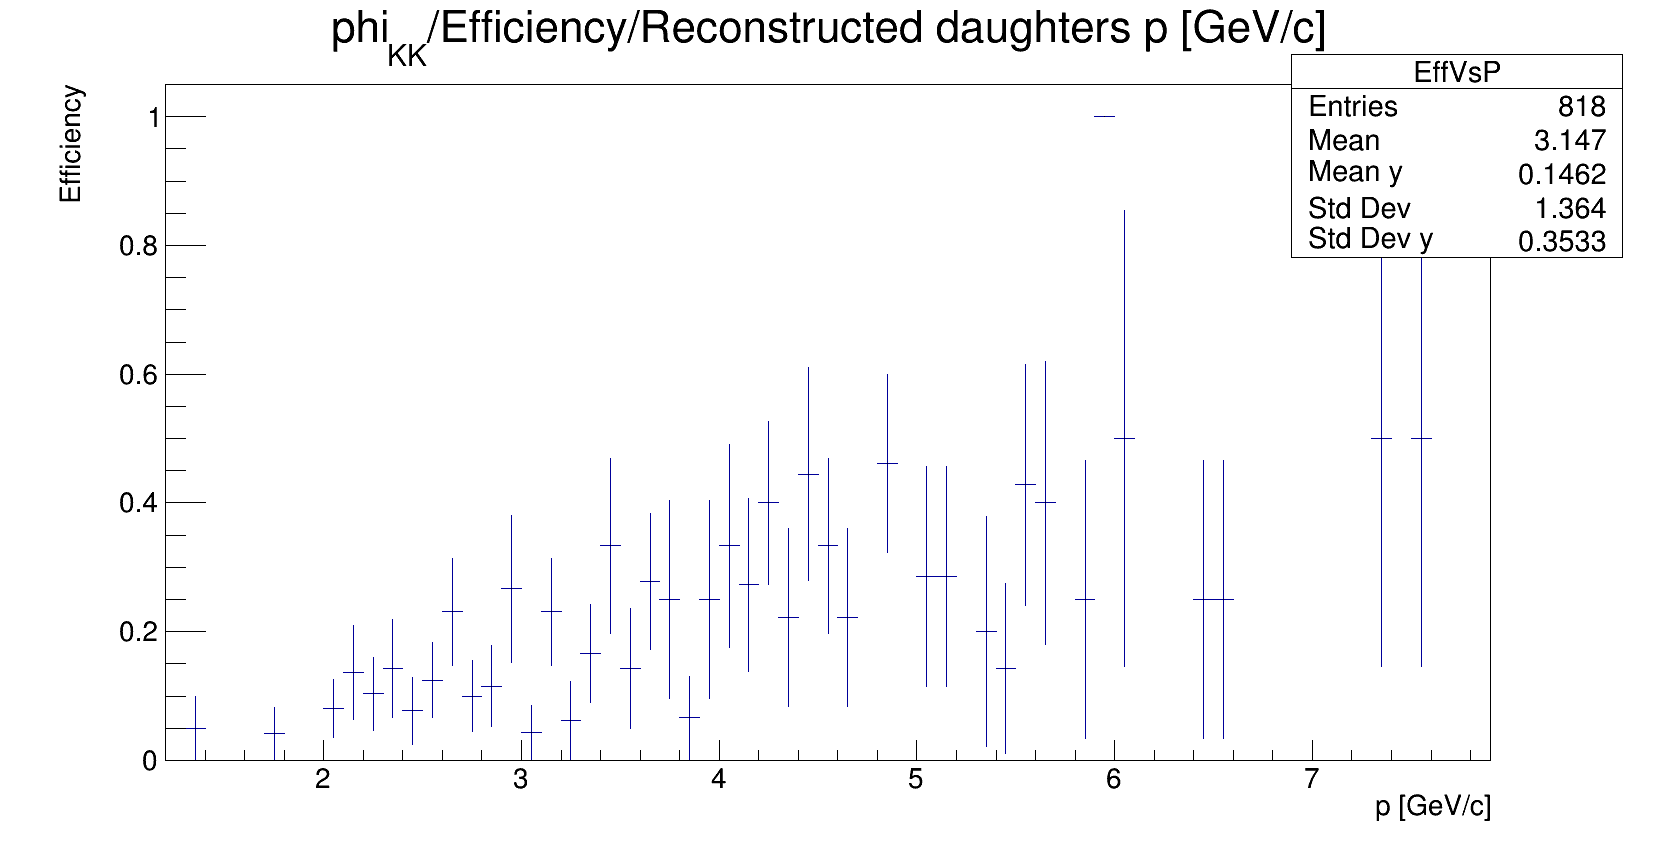
\includegraphics[width=0.5\textwidth]{reconstructed_eff_phi2500.png}
\end{figure}
\par Könnyű megtalálni azokat a részecskéket is amikké a $\Phi$-mezonok elbomlottak. Így találhatunk a bomlástermékek között
pionokat, kaonokat, $K^{0}_{S}$ részecskéket. 
\begin{figure}[H]
	\centering
	\begin{subfigure}{0.49\textwidth}
		\centering
		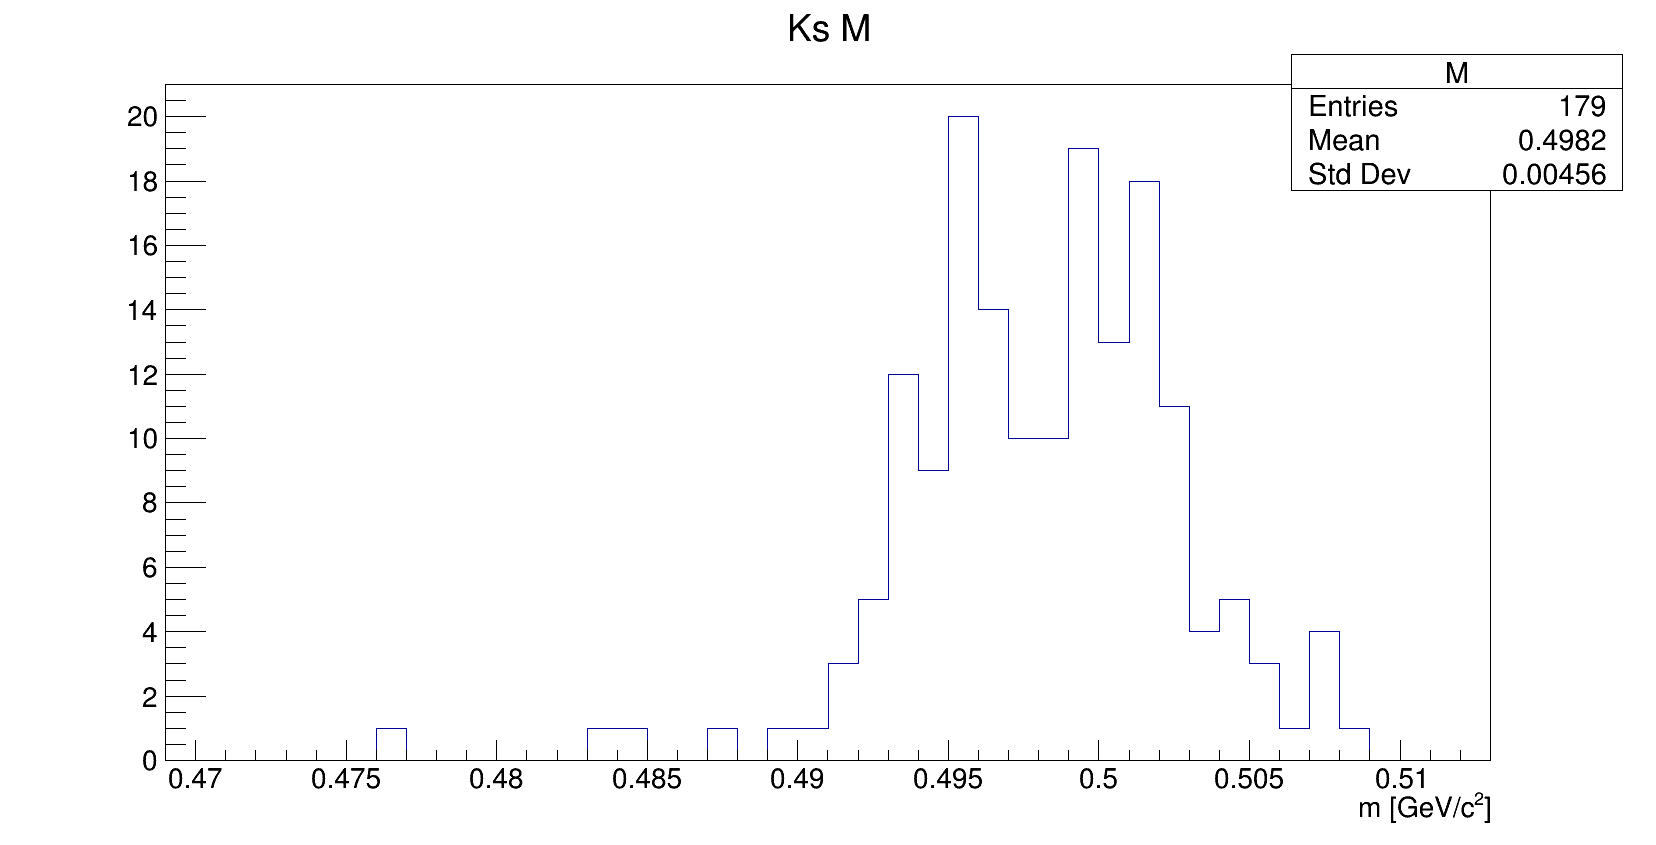
\includegraphics[width=0.95\textwidth]{kshort_phi2500.png}
		\caption{ $K^{0}_{S}$ részecskék }
	\end{subfigure}
	\begin{subfigure}{0.49\textwidth}
		\centering
		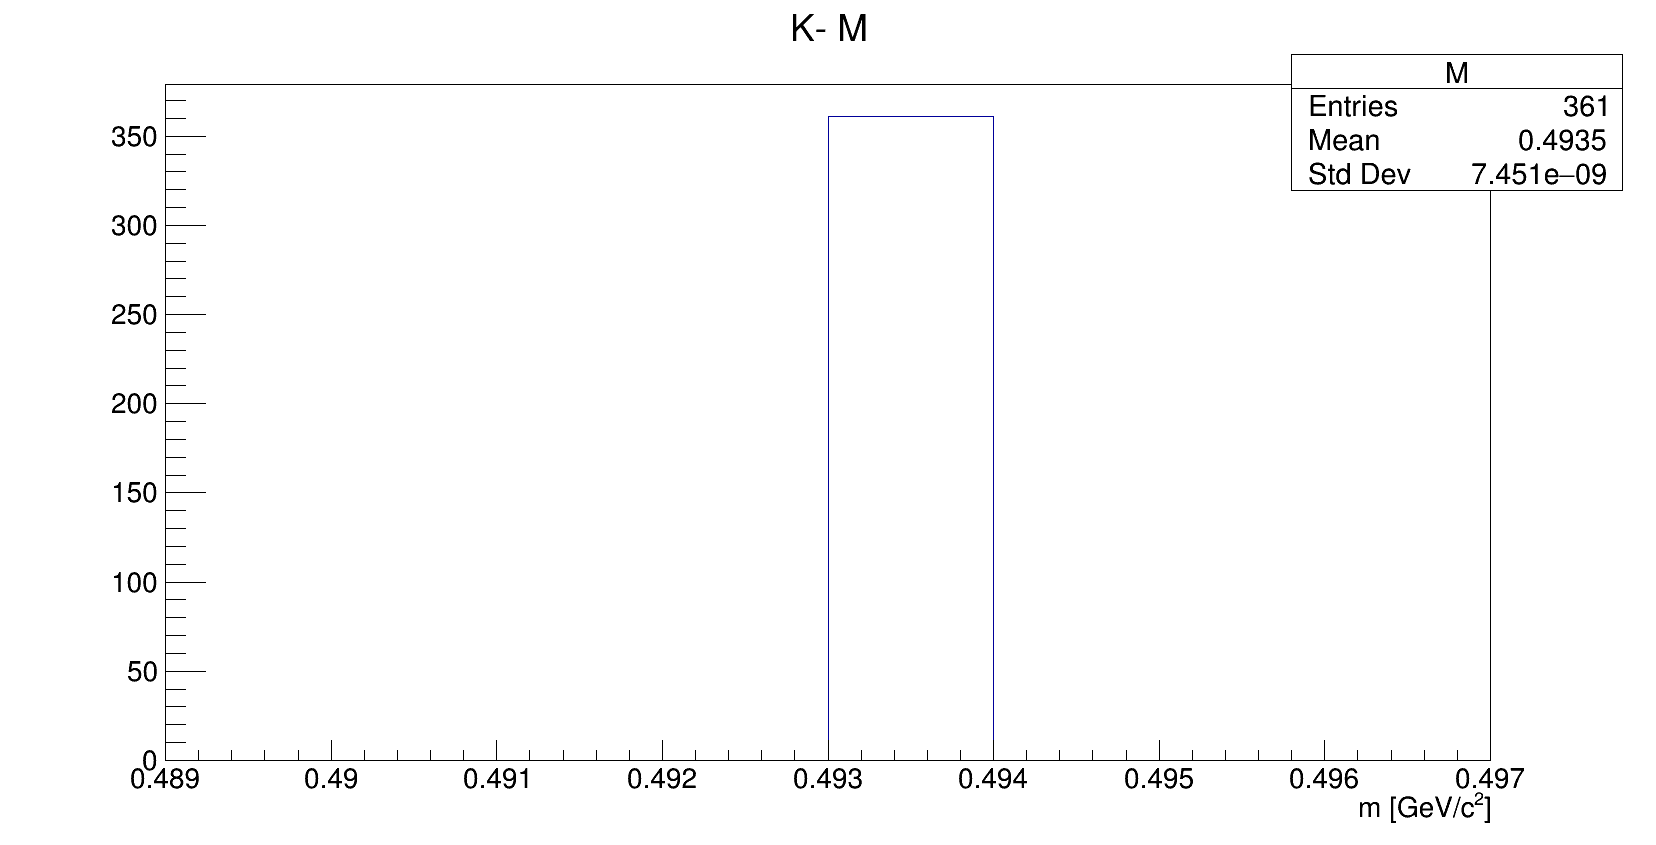
\includegraphics[width=0.95\textwidth]{k-_phi2500.png}
		\caption{ Negatív kaonok. }
	\end{subfigure}
\end{figure}
\par A pionokat itt nem tüntettem fel külön, mivel egy ilyen folyamat során azok nem adnak informatív képet, lévén, hogy nem csak a 
$\Phi$-mezon tud úgy bomlani, hogy pion is van a bomlástermékek között, de a kaonok és egyéb részecskék is, így a pionok multiplicitása igen
nagy.
\subsection{ Összegzés}
\vspace{5mm}
\par A CBM detektor képes lesz arra, hogy felismerje és megtalálja a $\Phi$-mezon bomlásokat, ezáltal a strange termelődést és a 
partonikus anyagot vizsgálni tudja. A szimulációk azt sugallják, hogy a detektor minden valószínűség szerint képes lesz detektálni a 
szükséges részecskéket a megfelelő hatásfokokkal.
\section{ Nehézion fizika itthon }
\vspace{5mm}
\par A Wigner Fizikai Kutatóközpontban dolgozó témavezetőmtől, Wolf Györgytől azt a feladatot kaptam, hogy az általa írt nehézion reakciós
programhoz írjak egy klaszterező programot. Ez a szimuláció a korábban említett, PHSD és UrQMD modellekhez hasonló, hazai fejlesztésű
projekt. A hadron-mag és mag-mag reakciókat transzport-egyenletek segítségével vizsgálva, a BUU-modell\footnote{Boltzmann-Uehling-Uhlenbeck modell}
felhasználásával egy időfüggő, részecskék kölcsönhatását figyelembe vevő modell segítségével szimulálja ez a program.
\par Ennek kimenetén többek között szerepelhetnek bizonyos részecskék és azok momentum- és térbeli eloszlása. Detektortól függően
máshogy lehet ezeket mérni. Ha olyan detektorunk van, ami csak töltött részecskéket mér, és a töltés nagyságát nem, akkor figyelembe
kell vennünk, ha például térbeli (vagy impulzustérbeli) közelség miatt csak egy beütést kapunk. Így az én programom pontosan arra képes, hogy
euklideszi-térben (vagy impulzustérben) klasztereket keres. Így a beütésszámra pontosabb jóslatot lehet majd adni tényleges detektor
környezetben.
\subsection{ Az algoritmus}
\par Nem tökéletesítettem még a programot, ha későbbiekben erre igény van természetesen fejlesztem. Egyenlőre hely- és impulzus-koordinátákat
olvas be, majd ezután próbálja meg klaszterezni a részecskéket. A klaszterezéshez nem a legjobban ismert klaszterező algoritmust
használtam hanem az úgynevezett minimális feszítő fa ( vagy MST \footnote{Minimal Spanning Tree} a későbbiekben ) algoritmust. Ezt egy 
gráfban a lehető legrövidebb utat találja meg. Két pont akkor van összekötve a gráfban, ha egy adott minimum távolságnál közelebb vannak.
Természetesen ez a minimális távolság is a bemenetről állítható. Egy részecske egy klaszter része, ha legalább az egyik részecskéhez a
klaszterben kellően közel van. 
\par Ennek az algoritmusnak talán az a legnagyobb előnye, hogy nem kell előre feltételezni, hogy hány klaszter van és azt sem, hogy 
azok vajon hol helyezkedhetnek el. Elméletben az algoritmus hatékonysága O($\log{m}\cdot n$) vagy O($\log{n}\cdot n + m$), ahol n a pontok
száma a gráfban, míg m az élek száma. A hatékonyság a használt adatstruktúráktól függ. Ez természetesen Prim algoritmusára \footnote{\url{https://en.wikipedia.org/wiki/Prim\%27s_algorithm}}
igaz, vannak ennél hatékonyabb megoldások is, de számomra ez tűnt a legkényelmesebb, legmegvalósíthatóbb választásnak. Továbbá egy francia 
kutatócsoport Nantes-ban hasonló nehézion fizikai szimulációjában is ezt az algoritmust javasolják.
\par  Az egyik elméleti nehézség a megvalósítás során az volt, hogy az algoritmus képes legyen több klasztert formálni. Hiszen miután 
nem tud továbbhaladni egy klaszterben, azaz nem tud több pontot hozzáadni, ki kell venni az adathalmazból a klaszterezett pontokat. Ezután lehet csak választani egy random pontot újra, és lefuttatni az eddigi algoritmust a már redukált gráfon.
\subsection{ A kód}
\par A kódot mellékelem, ezután beszélek majd a bemenetéről és kimenetéről.
\lstinputlisting[language=C++]{main.cpp}
\subsubsection{ Bemeneti paraméterek}
\par A program parancssorról működik.  Három paramétert vár a futás során. Az első paraméter a bemeneti fájl neve, a második a maximális 
klaszeterezési távolság, azaz a maximálisan definiálható élhossz két pont között. A harmadik paraméter pedig a kimeneti fájl neve, ami
egyesével listázza majd a klaszeterek méreteit és az összes klaszterek számát. A program képernyőre írja a gráf elkészítésének idejét
és a klaszterezés idejét is $ms$-ban. Ezt parancssorról át lehet irányítani egy tetszőleges fájlba ( >> time.dat ).
\par A bemeneti fájl formátuma adott. Ebben részecske adatok szerepelnek, és adott időlépésenként haladva követjük végig a részecskéket.
Sorénként a következő adatokat kapjuk: nukleon (igen/nem), töltés, tömeg(GeV), px, py, pz (GeV/c), rx, ry, rz (fm), ütközések száma.
\begin{lstlisting}
  1  1  0.938300 -0.177627  0.025891 -0.077826 -7.935590  0.056308-11.041818   1
  1  1  0.938300  0.418485  0.316837  0.882886 12.817832  5.254027  6.157795   2
  1  1  0.938300 -0.247703  0.057946 -0.044372-12.626606  4.831421-19.696069   1
  1  1  0.938300 -0.022614 -0.215107  0.223749 -4.957242 -6.073233 -4.840523   2
  1  1  0.938300 -0.208557 -0.300033  0.080906 -5.851900-14.546136-11.728940   4
  1  0  0.938300 -0.556290  0.208243  0.389433-16.943628 12.829147 -3.252291   7
  1  1  0.938300 -0.045176 -0.188415  0.277124 -3.621005 -9.789178 -6.976719   3
  1  1  0.938300 -0.562875 -0.475173  0.274616-17.897499-17.592449 -6.268526   3
  1  1  0.938300 -0.032136 -0.021516 -0.007764 -5.412685  0.558902-15.674200   1
\end{lstlisting}
\par Három szimulációs fájlt kaptam, mindegyik más időpillanatban állt meg. Az első 40 fm/c után, a második 50 fm/c, a harmadik pedig 60 fm/c
idő után. A fájlok 100 eseményt tárolnak, mindegyikben 394 db nukleon szerepel. Az ütközések 3 fm-es impakt paraméterrel játszódtak le. A részecskék
távolságának definícióját még tökéletesíteni kell. Először is elvégeztem egy klaszterezést külön térben és impulzus térben:
\subsection{ Távolság függés}
\par Valamelyik eseményre elvégezve a klaszterezési távolságtól való függés vizsgálatát a következőket kaptam.
\begin{figure}[H]
	\centering
	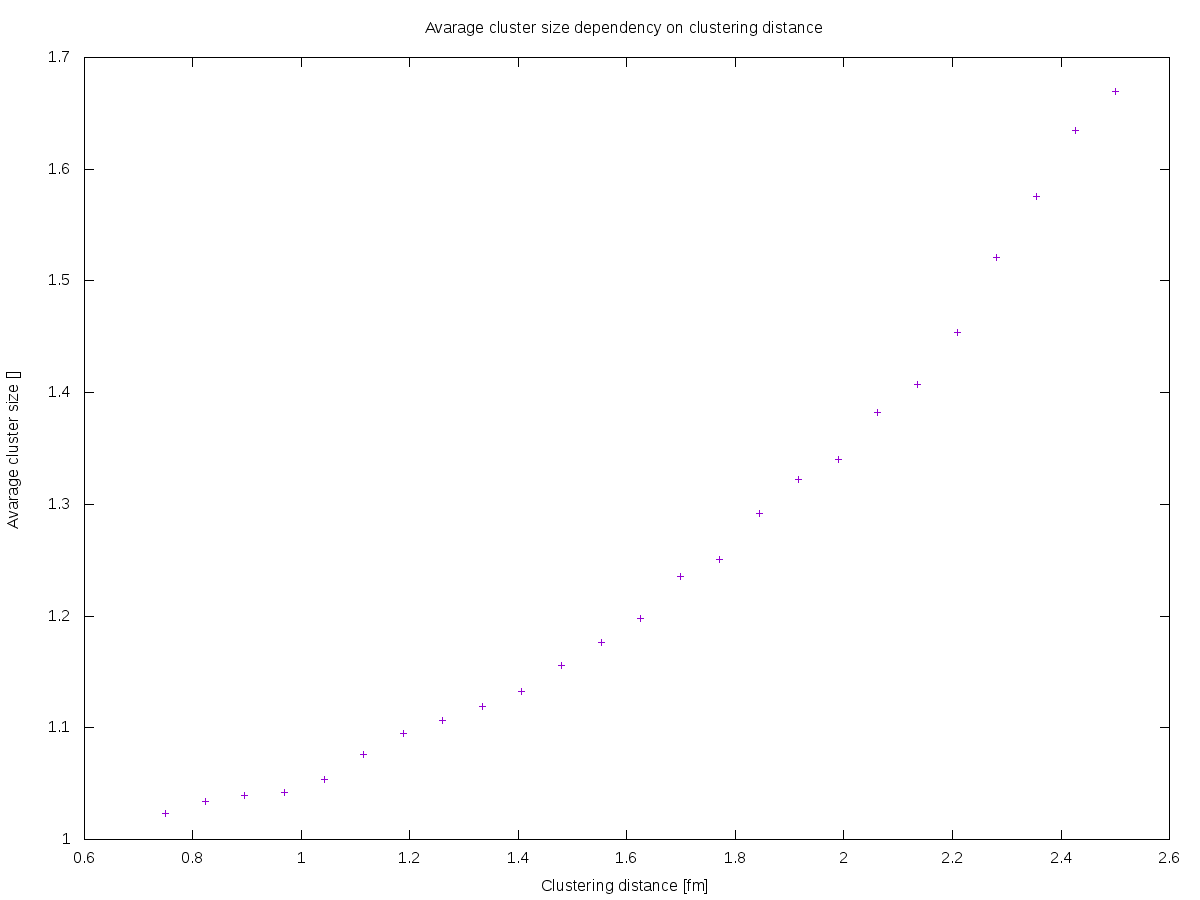
\includegraphics[width=0.7\textwidth]{dist-mean.png}
	\caption{ Térbeli klaszterezés eredménye. Klaszterezési távolság - átlagos klaszterméret }
\end{figure}
\par A számolást természetesen térbeli, és impulzustérbeli klaszterezésre is elvégeztem.
\begin{figure}[H]
	\centering
	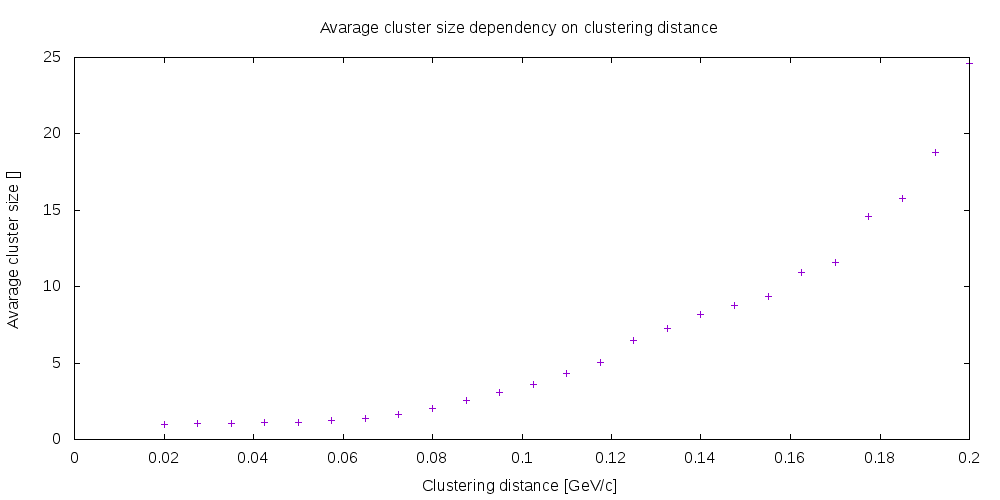
\includegraphics[width=0.7\textwidth]{momdist-mean.png}
	\caption{ Impulzustérbeli klaszterezés eredménye. Klaszterezési távolság - maximális klaszterméret }
\end{figure}
\par Térben a klaszterezés életképes, ha a távolság a részecskék között 1 fm alatt van, míg impulzustérben ez az érték 0.08 GeV/c alatti. Így jól látható,
hogy az impulzustérbeli távolság nagyjából egy nagyságrenddel kisebb, mint a térbeli távolság. Az előbbi klaszterezések még a kód korábbi verziójával
készültek, ez megtalálható a GitHub profilom alatt \footnote{github link}. Ahhoz, hogy ténylegesen összeálljanak a részecskék az kell, hogy mind térben,
mind impulzustérben közel legyenek egymáshoz. Ehhez felvettem egy olyan vektort aminek az első 3 komponense a térbeli koordinátákat tartalmazza,
második három komponenese az impulzustérbeli koordinátákat és ezeket beszoroztam egy $scalingFactor$-ral, hogy kompenzáljak a nagyságrendi különbség
miatt. Ezután különböző klaszterezési távolságkora, amelyek lineárisan nőttek lefuttattam a klaszterezést a 100 adatsorra és ebből készítettem eloszlás
hiszrogrammokat.
\par Az klaszterméret eloszlások változása a klaszterező távolság növekedésével rendere 40, 50, 60 fm/c után:
\begin{figure}[H]
	\centering
	\begin{subfigure}{.45\textwidth}
		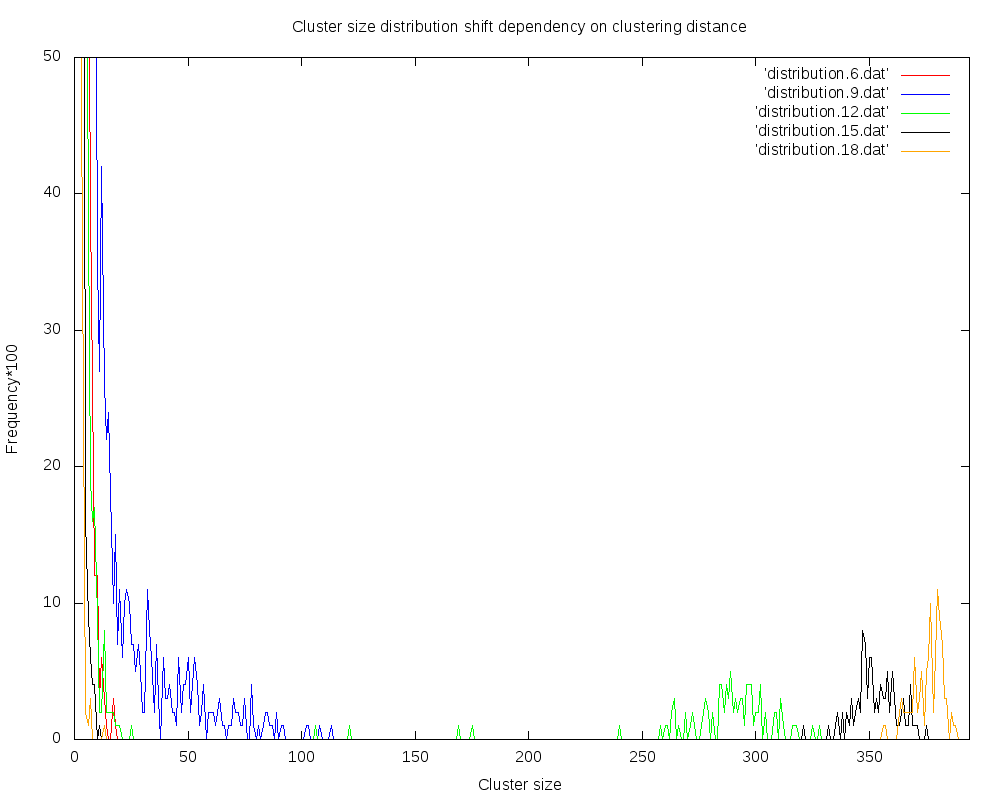
\includegraphics[width=0.96\textwidth]{ShiftInDistro80.png}
		\caption{ Klaszterszám - klaszterméret eloszlás 40 fm/c idő után }
	\end{subfigure}
	\begin{subfigure}{.45\textwidth}
		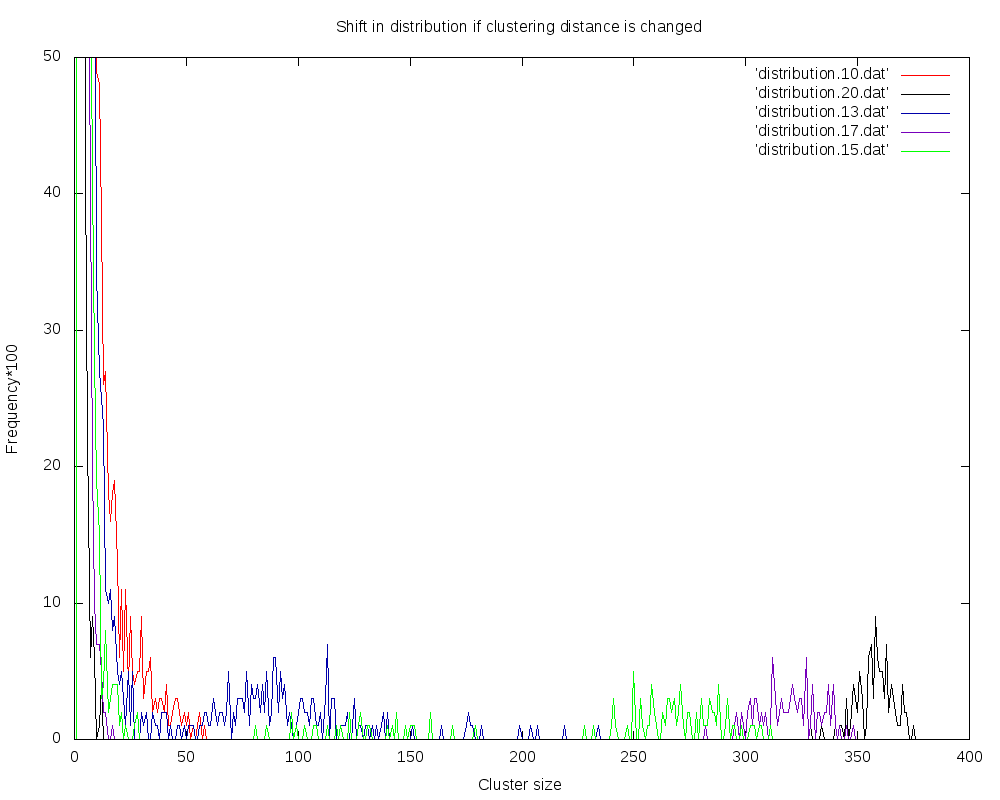
\includegraphics[width=.96\textwidth]{ShiftInDistro100.png}
		\caption{ Klaszterszám - klaszterméret eloszlás 50 fm/c idő után} 
	\end{subfigure}
\end{figure}
	\begin{figure}[H]
		\centering
		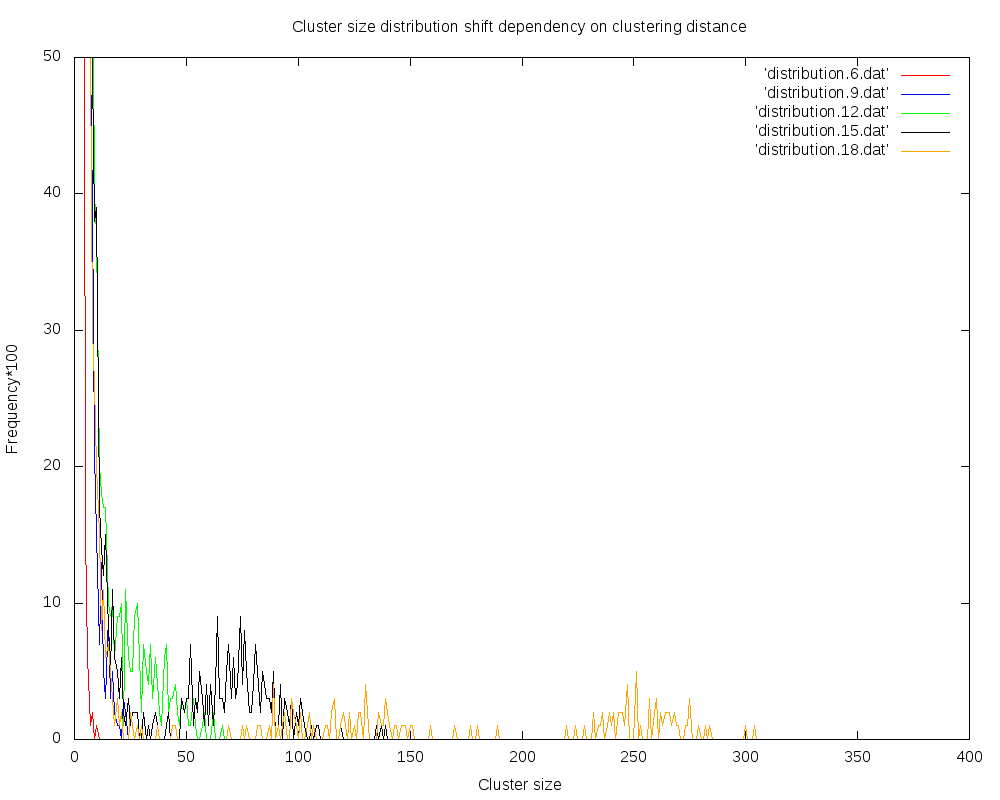
\includegraphics[width=0.65\textwidth]{ShiftInDistro120.png}
		\caption{ Klaszterszám - klaszterméret eloszlás 60 fm/c idő után} 
\end{figure}
\par Jól megfigyelhető, ahogy a klaszter távolság növelésével egyre gyakoriabbak lesznek a nagyméretű klaszterek. Ezek jelenthetnek nagyobb/kisebb
magokat. Szemléletes, például, hogy kis impakt paraméternél nagy számú 'törmelék' keletkezik, hiszen a 1/2 nukleonos klaszterek száma végig magas.
\par A továbbiakban vizsgáltam, hogy mi történik a klaszterező méret növelésével. Itt azt vizsgáltam, hogy az adott 100 párhuzamos fájlra nagyjából 
hasonló eredményeket kapok-e a klaszterezés után. Ezt úgy állapítottam meg, hogy felvettem egy diagramot aminek vízszintes tengelyén az átlagos 
klaszterméret, függőleges tengelyén pedig a maximum klaszter méret szerepelt mindegyik fájlra. Ez 100 pontot jelent a diagrammon. Ha ezt ábrázolom
akkor hasonló eredmény az, ha adott pontcsoportok nagyjából egy helyre koncentrálódnak, hiszen ezek részecske csoportosulásokat jelentenek. Elnyújtott
formájuk amiatt lehet, mivel az 1/2 részecskés klaszterek száma nagyon nagy. Ennél pontosabb definíciót nem fogok adni, mivel a távolság számítása
ebben kulcsfontossága és azon még javítanom kell a későbbiekben. Különböző, egyre növekedő klaszterező távolságokra az eredeményeim a következőek.
\par 40 fm/c esetén:
\begin{figure}[H]
	\centering
	\begin{subfigure}{.49\textwidth}
		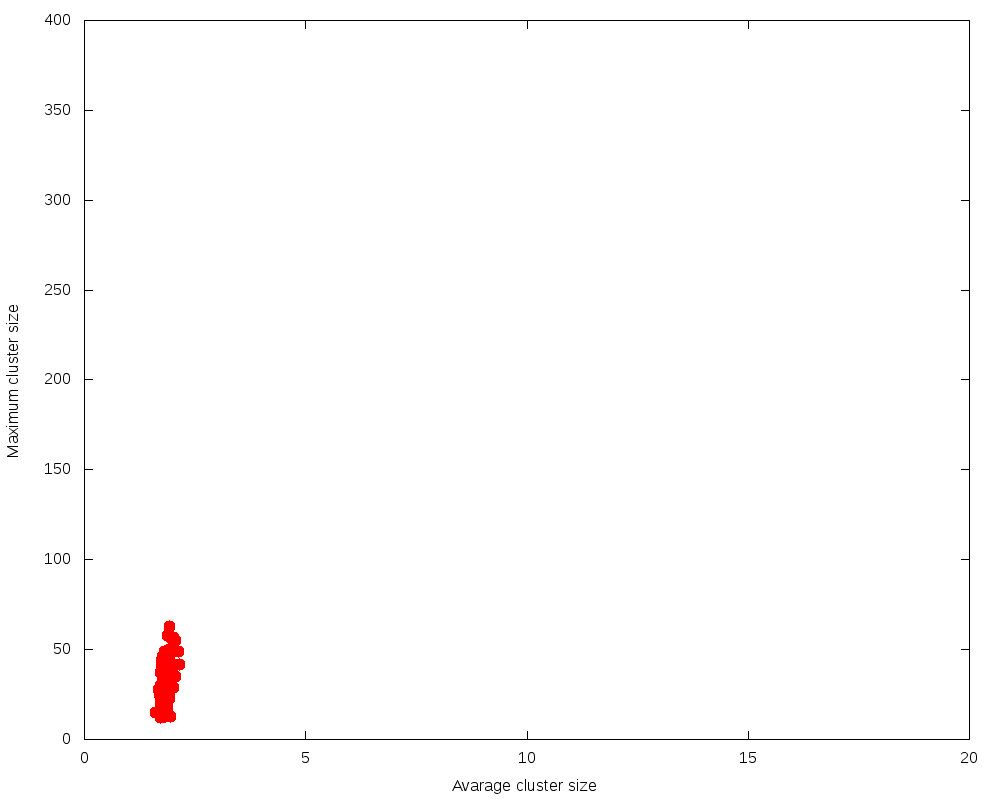
\includegraphics[width=0.92\textwidth]{mean-max8_80.png}
		\caption{ Átlagos klaszterméret - Maxmimális klaszterméret diagram }
	\end{subfigure}
	\begin{subfigure}{.49\textwidth}
		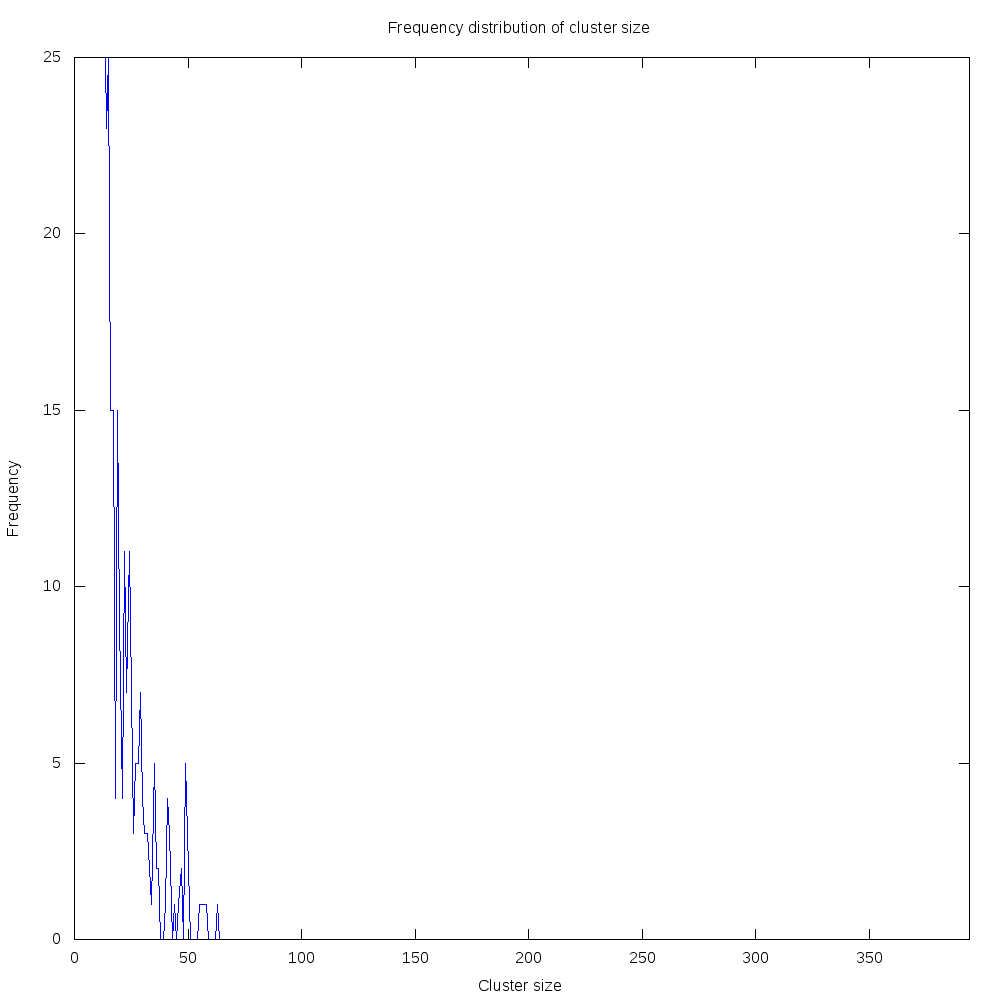
\includegraphics[width=.92\textwidth]{distribution_zoomed_8_80.png}
		\caption{ Klaszterméret eloszlás 100 eseményből } 
	\end{subfigure}
\end{figure}
\begin{figure}[H]
	\centering
	\begin{subfigure}{.49\textwidth}
		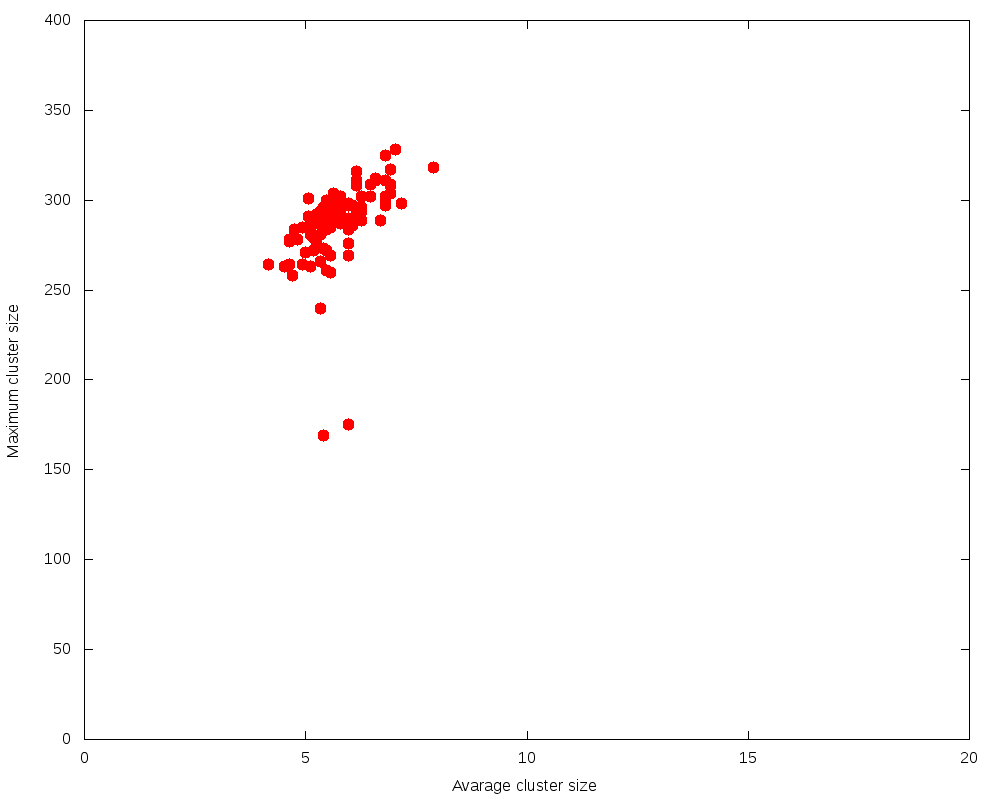
\includegraphics[width=0.92\textwidth]{mean-max12_80.png}
		\caption{ Átlagos klaszterméret - Maxmimális klaszterméret diagram }
	\end{subfigure}
	\begin{subfigure}{.49\textwidth}
		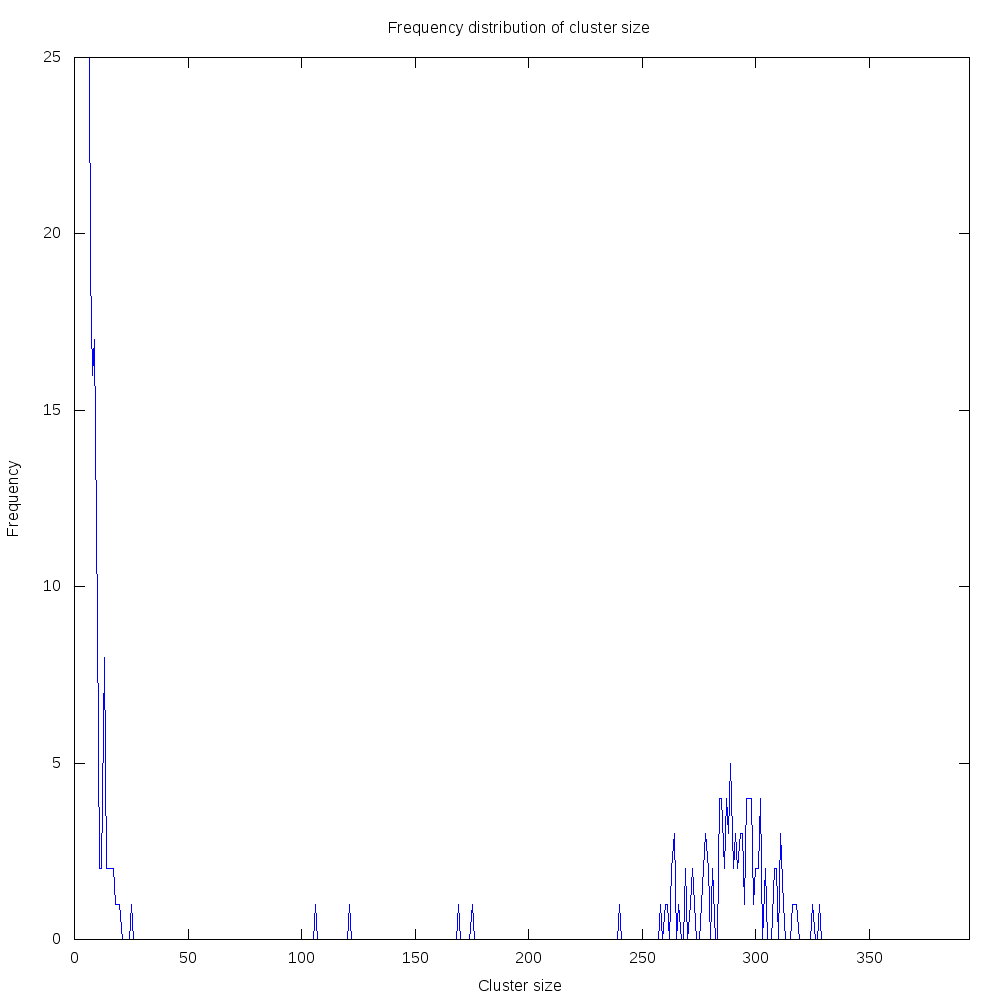
\includegraphics[width=.92\textwidth]{distribution_zoomed_12_80.png}
		\caption{ Klaszterméret eloszlás 100 eseményből } 
	\end{subfigure}
\end{figure}
\par Látható az eloszlásban történő eltolódás és az is, hogy az események nagyjából hasonlóak. 
\par 50 fm/c esetén:
\begin{figure}[H]
	\centering
	\begin{subfigure}{.49\textwidth}
		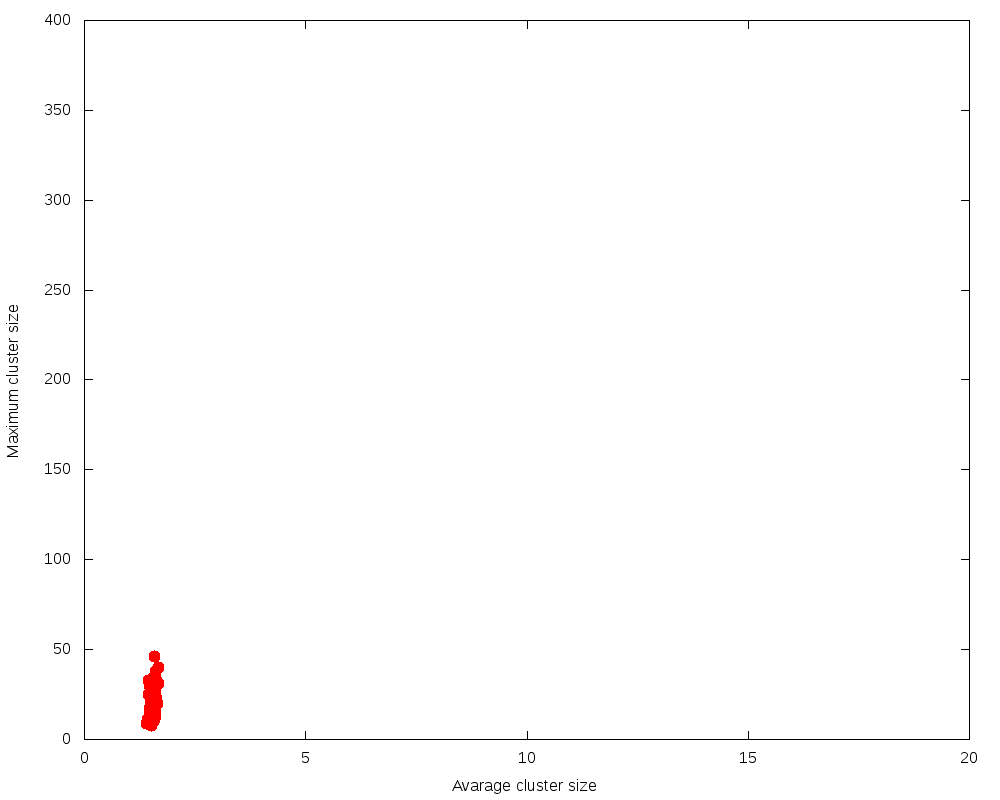
\includegraphics[width=0.92\textwidth]{mean-max9_100.png}
		\caption{ Átlagos klaszterméret - Maxmimális klaszterméret diagram }
	\end{subfigure}
	\begin{subfigure}{.49\textwidth}
		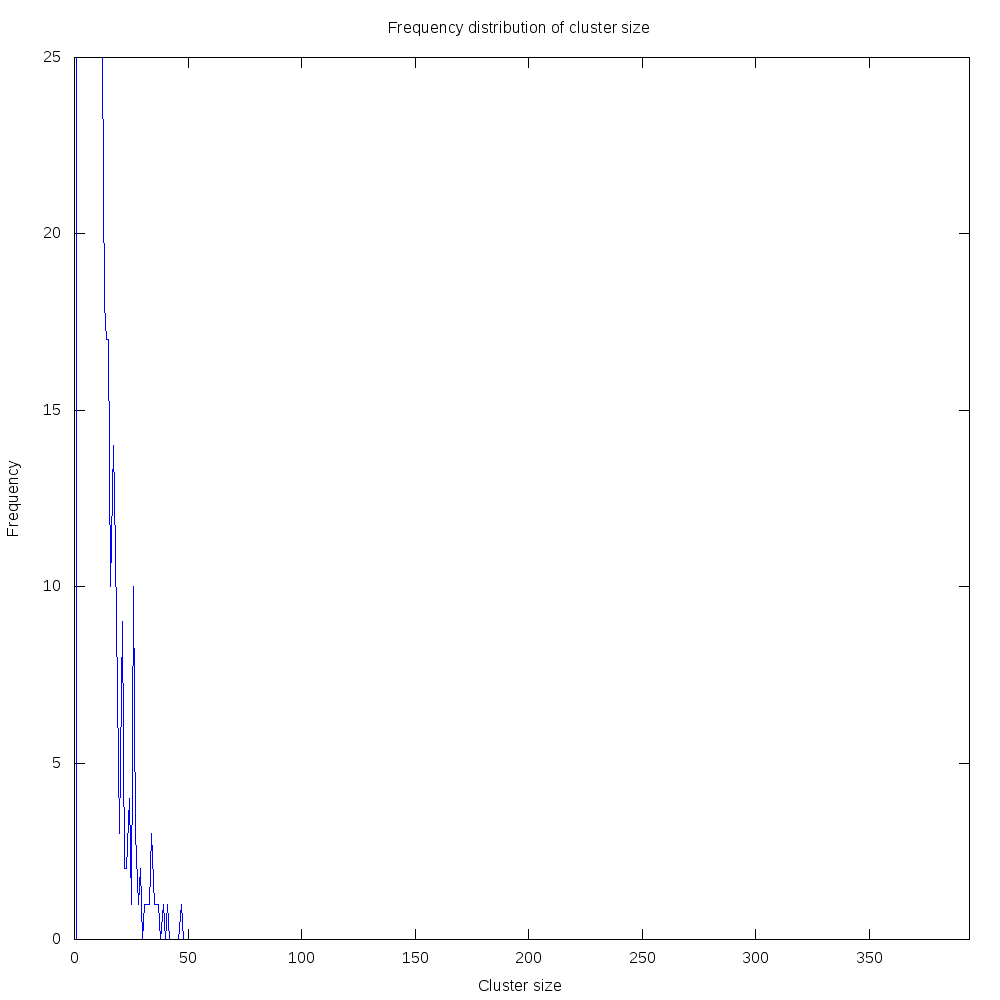
\includegraphics[width=.92\textwidth]{distribution_zoomed_9_100.png}
		\caption{ Klaszterméret eloszlás 100 eseményből } 
	\end{subfigure}
\end{figure}
\begin{figure}[H]
	\centering
	\begin{subfigure}{.49\textwidth}
		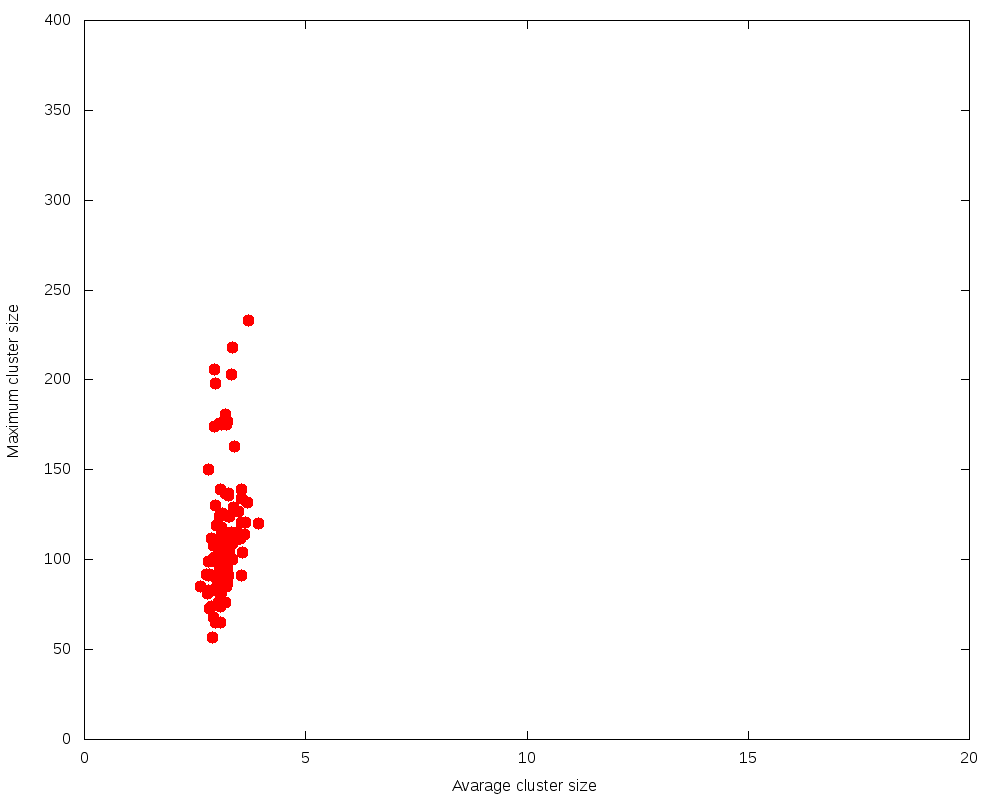
\includegraphics[width=0.92\textwidth]{mean-max13_100.png}
		\caption{ Átlagos klaszterméret - Maxmimális klaszterméret diagram }
	\end{subfigure}
	\begin{subfigure}{.49\textwidth}
		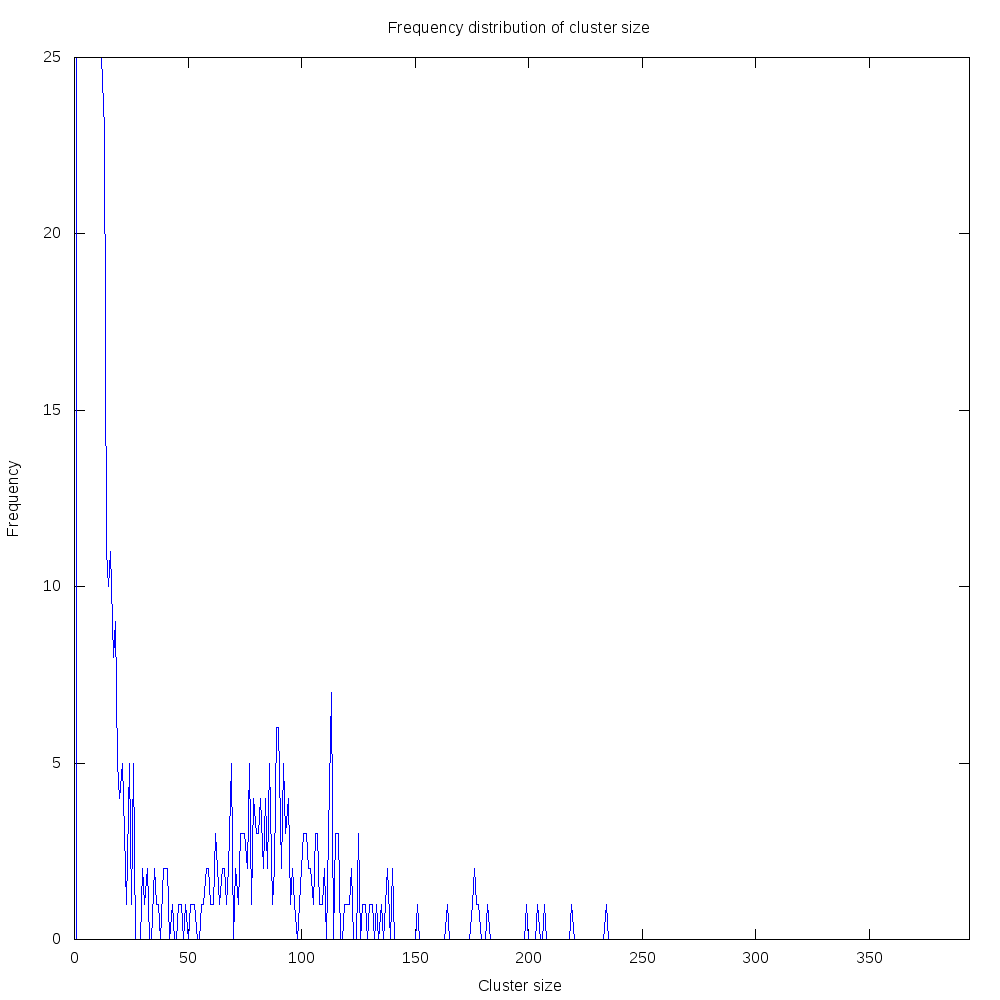
\includegraphics[width=.92\textwidth]{distribution_zoomed_13_100.png}
		\caption{ Klaszterméret eloszlás 100 eseményből } 
	\end{subfigure}
\end{figure}
\begin{figure}[H]
	\centering
	\begin{subfigure}{.49\textwidth}
		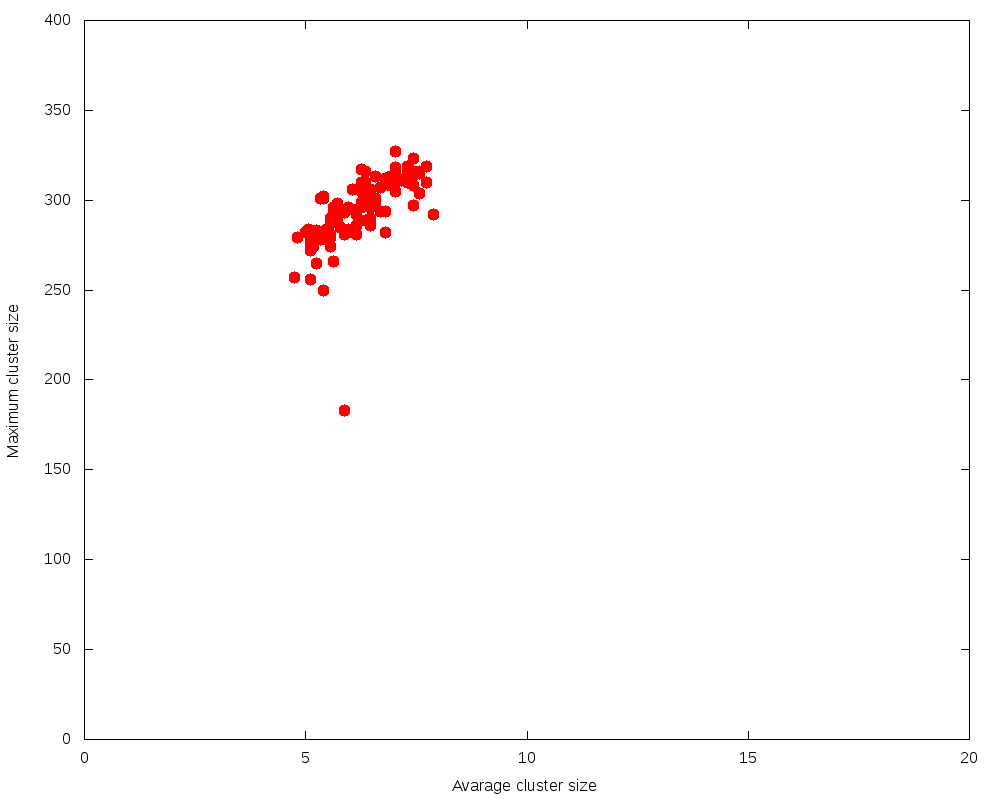
\includegraphics[width=0.92\textwidth]{mean-max16_100.png}
		\caption{ Átlagos klaszterméret - Maxmimális klaszterméret diagram }
	\end{subfigure}
	\begin{subfigure}{.49\textwidth}
		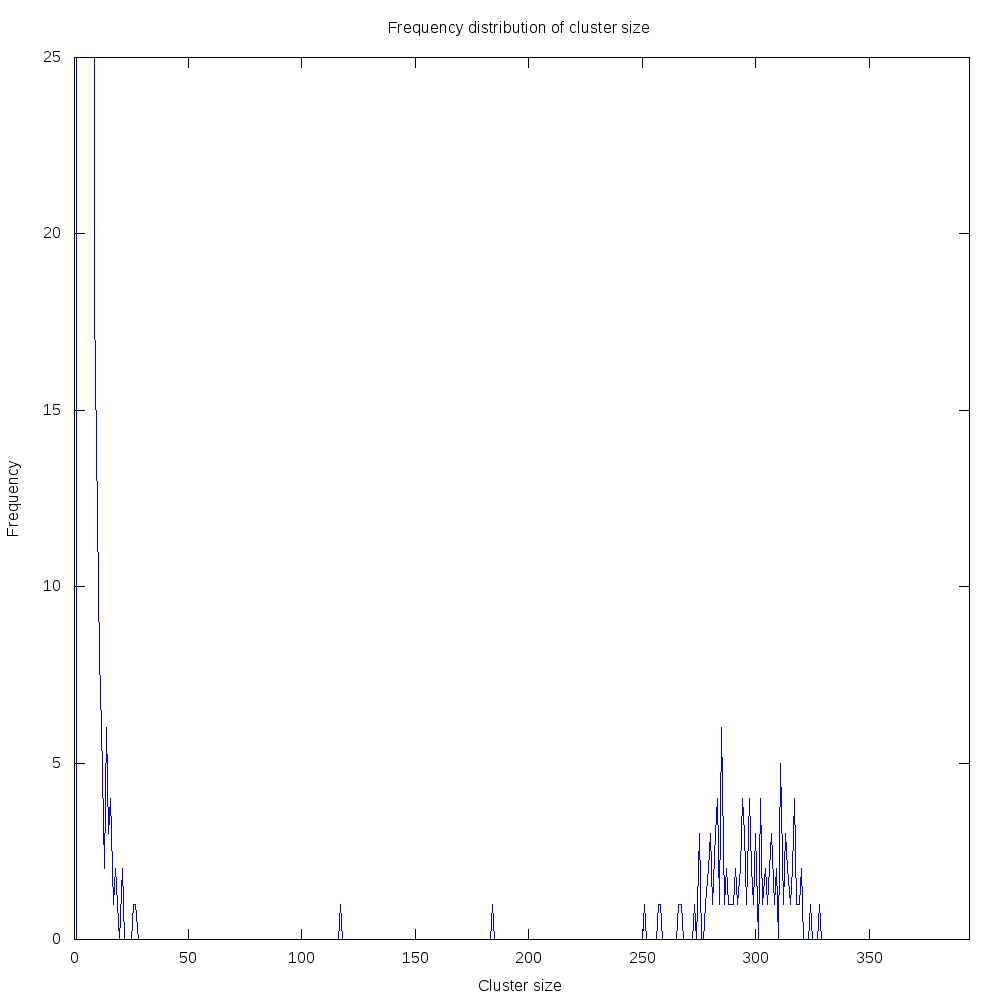
\includegraphics[width=.92\textwidth]{distribution_zoomed_16_100.png}
		\caption{ Klaszterméret eloszlás 100 eseményből } 
	\end{subfigure}
\end{figure}
\par Itt már a második diagramon jól látszik, hogy kezd szétválni a ponthalmaz két részre. A következő esetben már ez sokkal jobban 
látszik majd.
\par 60 fm/c esetén:
\begin{figure}[H]
	\centering
	\begin{subfigure}{.49\textwidth}
		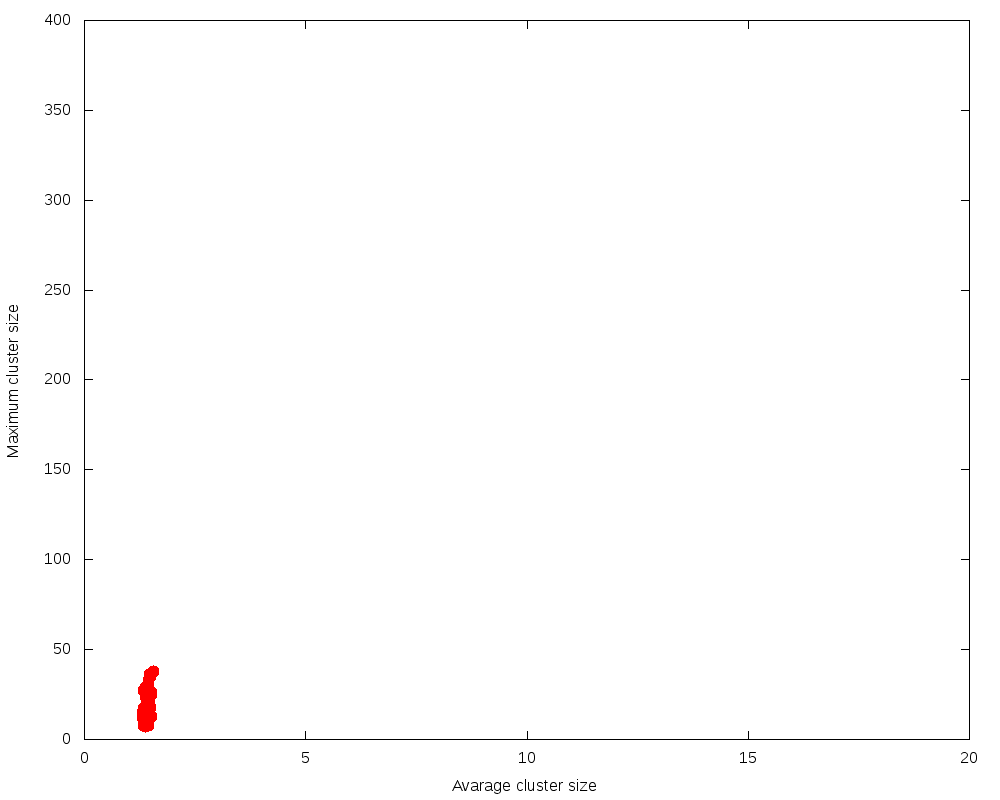
\includegraphics[width=0.92\textwidth]{mean-max10_120.png}
		\caption{ Átlagos klaszterméret - Maxmimális klaszterméret diagram }
	\end{subfigure}
	\begin{subfigure}{.49\textwidth}
		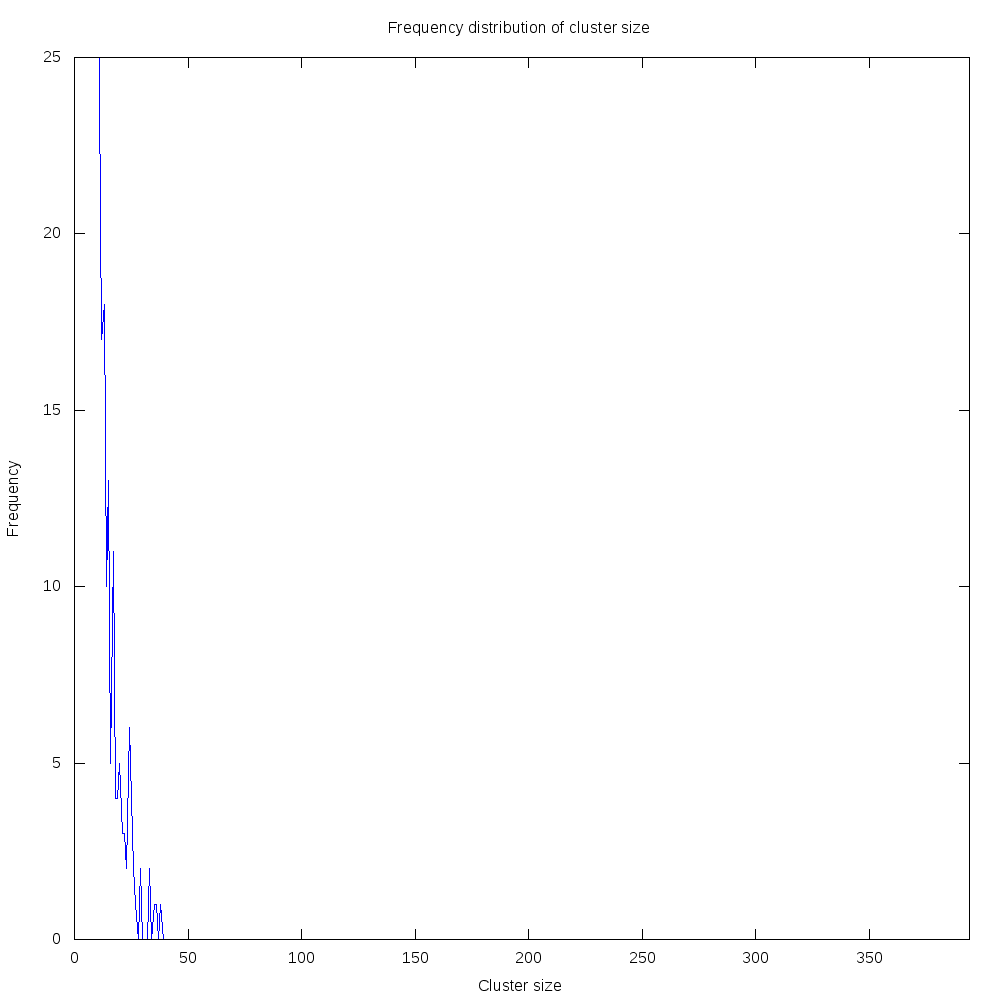
\includegraphics[width=.92\textwidth]{distribution_zoomed_10_120.png}
		\caption{ Klaszterméret eloszlás 100 eseményből } 
	\end{subfigure}
\end{figure}
\begin{figure}[H]
	\centering
	\begin{subfigure}{.49\textwidth}
		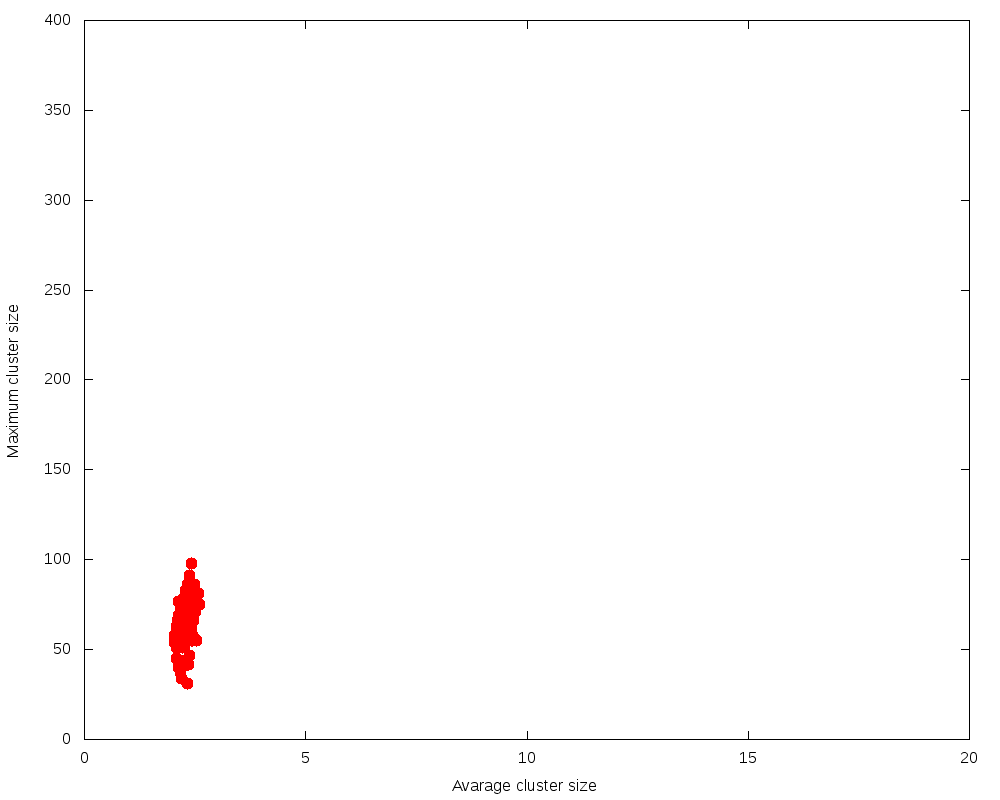
\includegraphics[width=0.92\textwidth]{mean-max14_120.png}
		\caption{ Átlagos klaszterméret - Maxmimális klaszterméret diagram }
	\end{subfigure}
	\begin{subfigure}{.49\textwidth}
		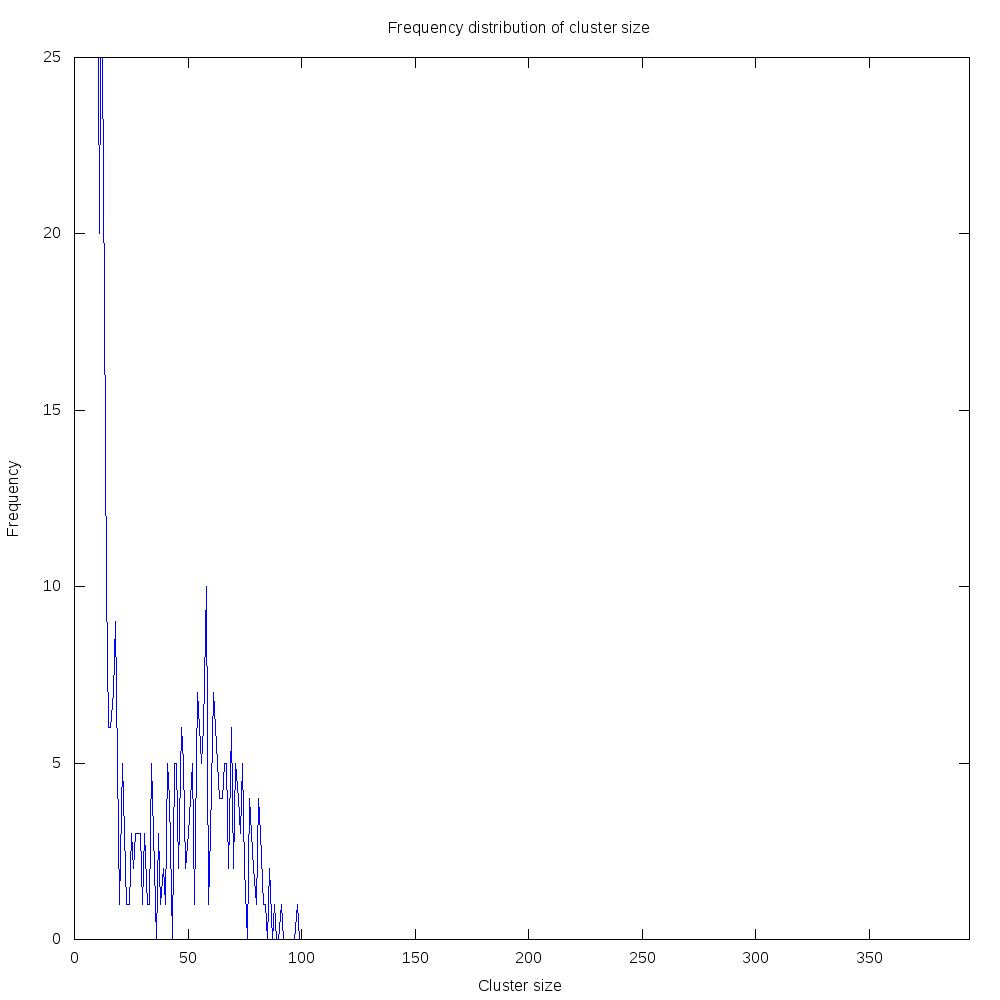
\includegraphics[width=.92\textwidth]{distribution_zoomed_14_120.png}
		\caption{ Klaszterméret eloszlás 100 eseményből } 
	\end{subfigure}
\end{figure}
\begin{figure}[H]
	\centering
	\begin{subfigure}{.49\textwidth}
		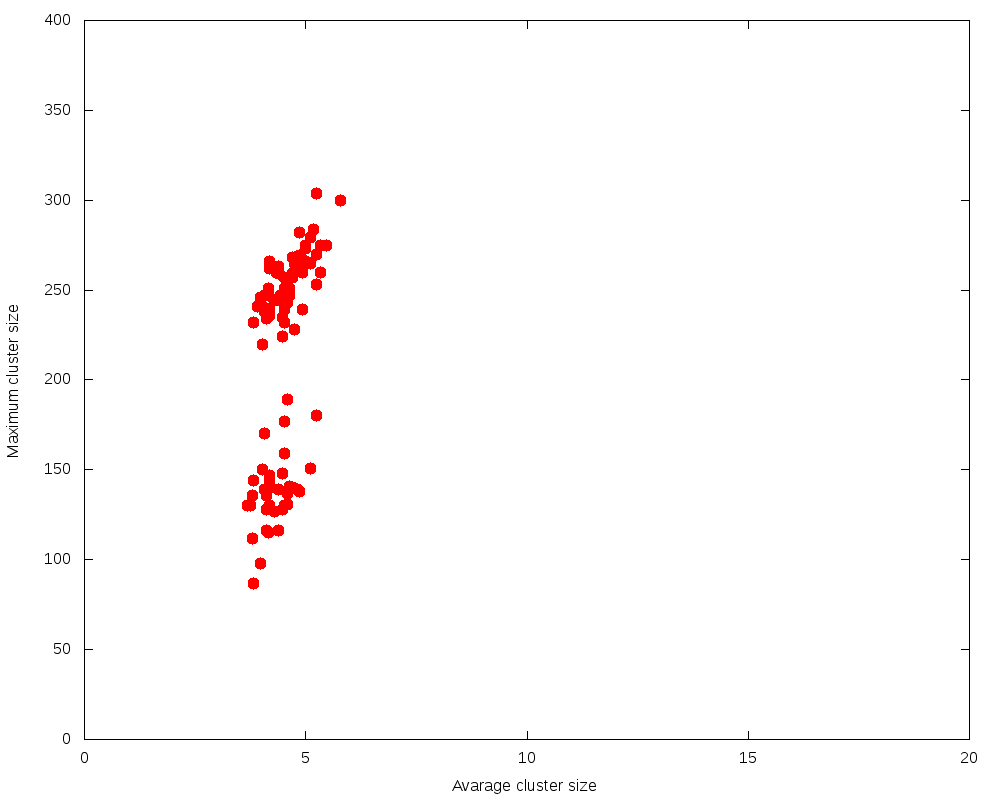
\includegraphics[width=0.92\textwidth]{mean-max18_120.png}
		\caption{ Átlagos klaszterméret - Maxmimális klaszterméret diagram }
	\end{subfigure}
	\begin{subfigure}{.49\textwidth}
		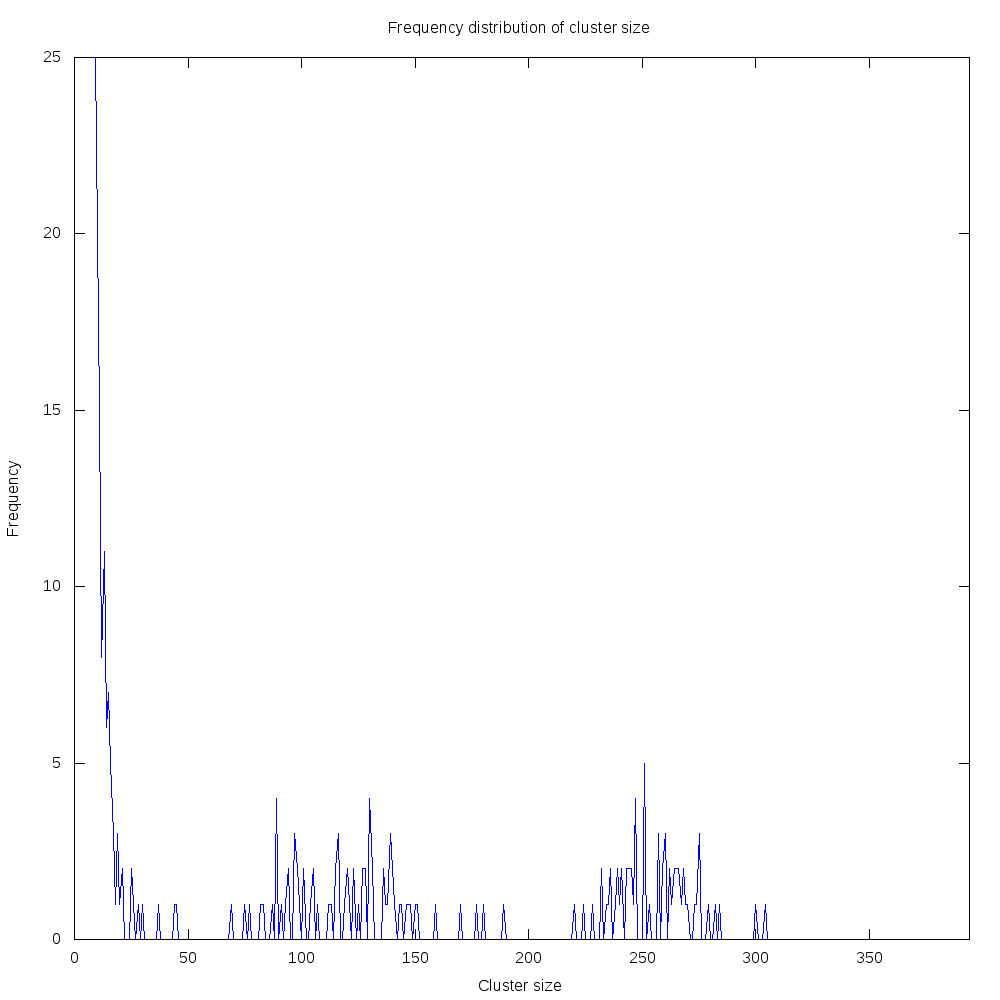
\includegraphics[width=.92\textwidth]{distribution_zoomed_18_120.png}
		\caption{ Klaszterméret eloszlás 100 eseményből } 
	\end{subfigure}
\end{figure}
\par Az utolsó (a) ábrán jól látszik, ahogy a ponthalmazok tükrözik az eloszlás diagrammot, amint az két jól elkülöníthető részre esik szét.
\subsection{ Kimenet}
\par A kimeneten tehát egy olyan fájlt kapunk, amiből meghatározható igen könnyen a maximális klaszterméret és az átlagos klaszterméret is.
Az fentebbi ábrákat is ezek alapján készítettem egy egyszerű programmal. Ezek mellett még külön fájlokban megkapjuk a klaszterek elemeit is
a program korábbi verziójában.
\subsection{ Sebesség, konklúzió}
\par A kód sebessége nagyban függ a definiált maximum távolságtól. Ha az előbbi algoritmust egy igen nagy szám,
akkor egy nagy klasztert találunk, viszonylag gyorsan, hiszen az MST keresés hiba nélkül lefut. Azonban minél nagyobb távolságokra is
éleket rakunk a kreált gráfba annál több számítást kell végeznünk és a sebesség nagyban leromlik. Lényegében mondható az, hogy a
klaszterezés belátható időn belül lefut tetszőlegesen nagy adathalmazra, hacsak a rendszer ki nem fogy a memóriából. 12 ezer sornyi adat 
klaszterezése esetén ez már megtörténhet. A program több dologra is képes mint amire jelenleg használva van. Az éleket tudja definiálni és
menteni is, ez az MST algoritmus sajátossága, de nekem nincs rá szükségem ebben az alkalmazásban. A távolság számítást módosítanom kell majd,
hiszen jelenleg csak euklideszi normám van, ami nem a legmegfelelőbb, de ez csak egy belső függvény átírást igényel majd. A kommentált kódrészletek 
a kimeneti fájlok emberi olvashatóságáért feleltek volna részben, valamint a további funkcionalitást kapcsoltam ki, de az adatok feldolgozása során
 kényelmesebb volt így eljárnom.
\begin{thebibliography}{9}
	\bibitem{CBMbook}
	Friman, Höhne, Knoll, Leupold, Randrup, Rapp, Senger
	\\\texttt{The CBM Physics Book - Compressed Baryonic Matter in Laboratory Experiments 2011 (Springer) Lect. Notes Phys.}
				
	\bibitem{phiALICE}
	 Tapia Takaki, J.D.
	 \\\texttt{ALICE Collaboration Journal of Physics G Nuclear Physics, 35, 044058 2008}
				
	\bibitem{CBMexp}
	 V.Vovchenko, I.Vassiliev, I.Kisel, M.Zyzak
	 \\\texttt{$\Phi$-meson production in Au+Au collisions and its feasibility in the CBM experiment, CBM Progress Report 2014}
				
	\bibitem{phiRICH}
	Bravina, L., Csernai, L., Faessler, A., et al. 2003, Nuclear Physics A, 715, 665 
				
	\bibitem{phiSTAR}
	F. Wang, R. Bossingham, Q. Li, I. Sakrejda,  N. Xu 
	\\\texttt{$\Phi$-meson reconstruction in the STAR TPC, 1998}
				
	\bibitem{cbmFAIR}
	Hans Rudolf Schmidt
	\\\texttt{Hyperons at CBM-FAIR, Journal of Physics: Conference Series 736}
\end{thebibliography}
\end{document}
